\documentclass[11pt]{article}

\usepackage{color, fullpage}

\usepackage[table]{xcolor}
\usepackage{makecell}

\usepackage{graphicx}

\usepackage{multicol}
\usepackage{calc}
\usepackage{tikz}
\usetikzlibrary{shapes.geometric, positioning, arrows.meta, calc, fit}
\usepackage{verbatimbox}

\usepackage{tcolorbox}
\tcbuselibrary{theorems}
\tcbuselibrary{fitting}

\usepackage[margin=0.5in]{geometry}
\usepackage{fancyvrb}

\graphicspath{{Pictures/}}

\usepackage{datetime}
\newdate{date}{28}{08}{2021}
\date{\displaydate{date}}

\usepackage{tocloft}
\renewcommand{\cftsecleader}{\cftdotfill{\cftsecdotsep}}
\renewcommand\cftsecdotsep{\cftdot}
%\renewcommand\cftsubsecdotsep{\cftdot}
\usepackage[hidelinks]{hyperref}

\title{CSCB07 Lecture Slides\thanks{Thanks to everyone in the CSCB07 Summer 2021 class.}}
\author{Vinesh Benny}




\begin{document}

\maketitle
\tableofcontents

\tikzset{
	method/.style = {
		minimum width=3cm,
		minimum height=0.5cm,
		draw,
		align=flush left,
		text width=2.7cm,
	},
	type/.style = {
		minimum width=3cm,
		draw,
		align=center,
		text width=2.7cm,
	}
}
\tikzset{frame/.style={line width=0.1mm, inner sep=0.9em, draw=#1}}
\definecolor{MVPBlue}{HTML}{5b9ad5}

\newpage
%\input{preamble.txt}
%
%\begin{document}
	\section{Version Control}

	\begin{itemize}
		\item Two flavours of Version Control
		\begin{itemize}
			\item Centralized (B07 uses this)
			\item Decentralized
		\end{itemize}

		\item Centralised Version
		\begin{itemize}
			\item Keep code in a centralized location (the “Repository”)
			\item Code in repository is the ``Master Copy" (\textbf{\underline{Never}} directly modify)
			\item Instead make local copies of the repository on each computer you will be working on (working copy)
			\item When major changes are made to local copy that you want to save, ``commit" change to repo
			\item Tools allow you to revert to a previous version of the source code (only when commits have occurred)
		\end{itemize}

		\item Some Terminology
			\vspace{\the\itemsep}
			\begin{itemize}
				\begin{minipage}[h]{\widthof{Repository/Repo} + 1cm}
					\item Repository/Repo
					\item Client program
				\end{minipage}
				\begin{minipage}[h]{\widthof{Working copy} + 1cm}
					\item Working copy
					\item Checkout
				\end{minipage}
				\begin{minipage}[h]{\widthof{Commit} + 1cm}
					\item Commit
					\item[\phantom{Fake item}] \phantom{text}
				\end{minipage}
			\end{itemize}



		\item Centralized systems include:
		\begin{itemize}
			\item \textbf{S}ub\textbf{V}ersio\textbf{n} (\textbf{SVN})
			\begin{itemize}
				\item SVN is the successor to \textbf{C}oncurrent \textbf{V}ersions \textbf{S}ystem (\textbf{CVS}), and was built to help fix many issues in CVS
			\end{itemize}
			\begin{minipage}[h]{\widthof{Mercurial} + 1cm}
				\item Git
				\item Mercurial
			\end{minipage}
			\vspace{\the\itemsep}
			\begin{minipage}[h]{\widthof{ClearCase} + 1cm}
				\item ClearCase
				\item Perforce
			\end{minipage}

		\end{itemize}

		\item SSH and SCP are \textbf{not} version control systems
		\begin{itemize}
			\item \textbf{S}ecure \textbf{Sh}ell (SSH) is used to connect to a remote computer and work in a shell on that computer
			\item \textbf{S}ecure \textbf{C}o\textbf{p}y (SCP) is used to:
			\begin{itemize}
				\item Securely copy files from one computer to another
				\item Transfer a copy of the files but does \textbf{not} version them
			\end{itemize}
		\end{itemize}

		\item Version Control – Managing Concurrency

		\emph{When two or more people want to edit the same file at the same time}
		\begin{itemize}
			\item Pessimistic concurrency
			\begin{itemize}
				\item Only allow one writeable copy of each file
				\item e.g. Microsoft Visual SourceSafe, Rational ClearCase
			\end{itemize}

			\item Optimistic concurrency
			\begin{itemize}
				\item Allow writes, fix issues afterwards
				\item Merging
				\begin{itemize}
					\item SVN is either able to merge without help from the user, or
					\item \textit{Conflict}: SVN needs the user to resolve the conflict
				\end{itemize}
				\item e.g. Subversion, CVS, Perforce
			\end{itemize}
			\newpage
			\item Optimistic Concurrency – Merging Options

			Select from: \textbf{(p)} postpone, \textbf{(df)} diff-full, \textbf{(e)} edit, \textbf{(mc)} mine-conflict, \textbf{(tc)} theirs-conflict and \textbf{(s)} show all options.\\[-15pt]
			\begin{center}
				\begin{minipage}[c]{0.6\textwidth}
					\begin{itemize}
						\item[(e) edit] - changed merged file in an editor
						\item[(df) diff-full] - show all changes made to merged file4
						\item[(r) resolved]  - accept merged version of file\\
						\item[(dc) display-conflict] - show all conflicts (ignoring merged version)
						\item[(mc) mine-conflict] -  accept my version for all conflicts (same as above)
						\item[(tc) theirs-conflict] -  accept their version for all conflicts (same as above) \\
						\item[(mf) mine-full] - accept my version of entire file (even non-conflicts)
						\item[(tf) theirs-full]  - accept my version of entire file (same as above)\\
						\item[(p) postpone] - mark the conflict to be stored later
						\item[(l) launch] - launch external tool to resolve conflict
						\item[(s) show all] - show this list
					\end{itemize}
				\end{minipage}
			\end{center}
		\end{itemize}

		\item Integrating the code - Reasons for merge conflicts\\[-15pt]
		\begin{itemize}
		\begin{minipage}[t]{\widthof{Experimental features being built} + 1cm}
				\item Communication
				\item Complex code bases
				\item Experimental features being built
		\end{minipage}
		\begin{minipage}[t]{\widthof{Two features being built in same class by different developers}}
				\item More than one project on the go that impacts this code
				\item Two features being built in same class by different developers
		\end{minipage}
		\end{itemize}

		\item Branching
		\begin{itemize}
			\item Branches are divergent copies of development lines
			\item These versions are used to build out complex features, or do experiments,
			without having an impact on the main code line
			\item Strategies include:
			\begin{itemize}
				\item No branching
				\item Release branching
				\item Feature branching
			\end{itemize}
		\end{itemize}

		\item Storage scheme
		\begin{itemize}
			\item Storing every copy of every file generated over the course of a project is not practical
			\item Version control systems store incremental differences in files/folder structures
			\item These differences store enough information to re-construct previous versions, without storing every single copy ever made of the file
		\end{itemize}

		\item What’s Stored Where
		\begin{itemize}
			\item Server side: out of scope
			\item Local copy contains a special directory, \textbf{.svn}
			\begin{itemize}
				\item It stores (locally) the information subversion needs to keep track of your files, version numbers, where the repository is, etc.
				\item Needless to say, you should not mess with the contents of this directory. Let subversion do its job
			\end{itemize}
		\end{itemize}

		\item General rules
		\begin{itemize}
			\item Update and commit frequently
			\item Never break the main branch
			\item Always comment clearly what changes are in a revision
			\item Test all code before accepting merge
			\item Communicate with your team!
		\end{itemize}
	\end{itemize}
%\end{document}
\newpage

\section{Introduction to Java}
\begin{itemize}

	\item What is Java?
	\begin{itemize}
		\item An object-oriented language invented by James Gosling in 1994 at Sun Microsystems
		\item Write once, run anywhere (WORA)
		\item Widely-used in industry
		\item Used to develop software running on:
		\begin{itemize}
			\begin{minipage}[t]{0.25\textwidth}
				\item Desktop Computers
			\end{minipage}
			\begin{minipage}[t]{0.15\textwidth}
				\item Servers
			\end{minipage}
			\begin{minipage}[t]{0.2\textwidth}
				\item Mobile devices
			\end{minipage}
		\end{itemize}
	\end{itemize}

	\item Java Programs
	\begin{enumerate}
		\item Writing the source code using a text editor
		\item Translating the source code into Java bytecode using a compiler
		\begin{itemize}
			\item Bytecode is similar to machine instructions but is architecture neutral and can run on any platform that has a Java Virtual Machine (JVM)
		\end{itemize}
		\item Executing the bytecode
		\begin{itemize}
			\item The JVM is an interpreter: it translates bytecode into the target machine language code one at a time rather than the whole program as a single unit
			\item Each step is executed immediately after it is translated\\[-21pt]
		\end{itemize}
	\end{enumerate}
	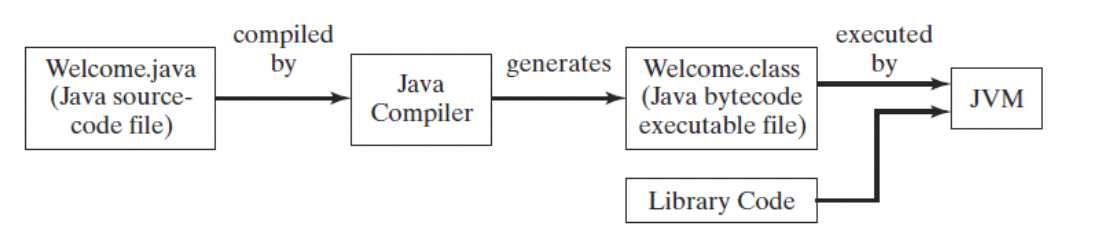
\includegraphics[scale=.75]{Compile flow.png}\\[-30pt]

	\item Integrated Development Environment
	\begin{itemize}
		\item A system comprising several tools that facilitate software development and testing
		\item Popular IDEs:
		\begin{itemize}
			\begin{minipage}[t]{0.15\textwidth}
				\item Eclipse
			\end{minipage}
			\begin{minipage}[t]{0.15\textwidth}
				\item NetBeans
			\end{minipage}
			\begin{minipage}[t]{0.2\textwidth}
				\item IntelliJ
			\end{minipage}
		\end{itemize}
	\end{itemize}

	\item Data Types
	\begin{itemize}
		\item Eight primitive types
		\begin{itemize}
			\item byte, char, short, int, long, float, double, boolean
		\end{itemize}
		\item Objects
		\begin{itemize}
			\item Defined using \textbf{classes}
			\item Java provides wrapper classes to use primitive types as objects (e.g. Integer, Double, etc)
		\end{itemize}
	\end{itemize}

	\item Numeric Primitive Types
	%	\includegraphics[scale=.7]{Primitive types.png}
	\begin{center}
		\begin{tabular}{ l l l }
			\hline
			\textit{Name} & \textit{Range} & \textit{Storage Size}\\
			\hline\\[-10pt]
			\textbf{byte} & $ -2^7 $ to $ 2^7 - 1 \, (-128 \text{ to } 127)  $  & 8-bit signed\\
			\textbf{short} & $ -2^{15} $ to $ 2^{15} - 1 \, (-32768 \text{ to } 32767)  $ & 16-bit signed\\
			\textbf{int} & $ -2^{31} $ to $ 2^{31} - 1 \, (-2147483648 \text{ to } 2147483647)  $ & 32-bit signed\\
			\textbf{long} & $ -2^{63} $ to $ 2^{63} - 1  $ & 64-bit signed\\
			& (i.e., $-9223372036854775808 \text{ to } 9223372036854775807$) & \\
			\textbf{float} & Negative range: $ -3.4028235\text{E} + 38$ to $ -1.4\text{E} -45$ & 32-bit IEEE 754\\
			& Positive range: $ 1.4\text{E} -45 $ to $ 3.4028235\text{E} + 38 $ & \\
			\textbf{double} & Negative range: $ -1.7976931348623137\text{E} + 38$ to $ -4.9\text{E} - 324$ & 64-bit IEEE 754\\
			& Positive range: $4.9\text{E} - 324$ to $1.7976931348623137\text{E} + 38$ &
		\end{tabular}
	\end{center}

	\item Classes
	\begin{itemize}
		\item A typical Java class includes the following:
		\begin{itemize}
			\item Data fields to represent the state of an object
			\item Methods to represent the behavior of an object. Each method has:
			\begin{itemize}
				\item A return type (\textbf{void} if nothing is returned)
				\item Zero or more arguments
			\end{itemize}
			\item Special type of methods, known as constructors, that perform initialization actions. A constructor:
			\begin{itemize}
				\item Has no return type (not even \textbf{void})
				\item Has zero or more arguments
				\item Should have the same name as the class
				\item Is invoked using the \textbf{new} operator
			\end{itemize}
		\end{itemize}
		\item Instantiation is creating an object (or an instance of a class)
	\end{itemize}

	\item The \textit{main} method
	\begin{itemize}
		\item The main method is the entry point where the program begins
		execution
		\item Should have the following form:
		\begin{Verbatim}
			public static void main(String [] args) {
				//write your code here
			}
		\end{Verbatim}
	\end{itemize}

	\item Default values
	\begin{itemize}
		\item The default value of a data field is:
		\begin{itemize}
			\begin{minipage}[t]{0.25\textwidth}
				\item \textbf{\textit{null}} for a reference type
			\end{minipage}
			\begin{minipage}[t]{0.25\textwidth}
				\item \textbf{0} for a numeric type
			\end{minipage}

			\begin{minipage}[t]{0.25\textwidth}
				\item \textbf{false} for a boolean type
			\end{minipage}
			\begin{minipage}[t]{0.25\textwidth}
				\item \textbf{`$\backslash$u0000'} for a char type
			\end{minipage}
		\end{itemize}
		\item Java assigns no default value to a local variable inside a method
	\end{itemize}

	\item Scope
	\begin{itemize}
		\item The scope of fields and methods is the entire class
		\item The scope of a local variable starts from its declaration until the end
		of the block that contains it
	\end{itemize}

	\item Differences between Variables of Primitive Types and Reference Types
	\begin{itemize}
		\item Every variable represents a memory location that holds a value
		\item For a variable of a primitive type, the value is of the primitive type
		\item For a variable of a reference type, the value is a reference to where an object is located (i.e. a pointer)
		\item When you assign one variable to another:
		\begin{itemize}
			\item For a variable of a primitive type, the real value of one variable is assigned to
			the other variable
			\item For a variable of a reference type, the reference of one variable is assigned to the other variable.
		\end{itemize}
	\end{itemize}

	\item The \textit{this} reference
	\begin{itemize}
		\item The \textbf{this} \textit{keyword} is the name of a reference that an object can use to
		refer to itself
		\item It can be used to reference the object’s instance members
	\end{itemize}

	\item The \textit{static} modifier
	\begin{itemize}
		\item Static fields/methods can be accessed from a reference variable or
		from their class name
		\item Non-static (or instance) fields/methods can only be accessed from a reference variable
	\end{itemize}

	\item Arrays
	\begin{itemize}
		\item An array is a data structure that represents a collection of the same types of data
		\item Once an array is created, its size is fixed
		\begin{itemize}
			\item e.g. \textbf{int [] A = new int[10];}
		\end{itemize}
		\item The size of an array A can be found using \textbf{A.length}
		\item When an array is created, its elements are assigned the default value
		\item Array elements could be initialized individually
		\begin{itemize}
			\item e.g. \textbf{A[0] = 5;}
		\end{itemize}
		\item Array initializer (combines declaration, creation, and initialization)
		\begin{itemize}
			\item e.g. \textbf{double[] myList = {1.9, 2.9, 3.4, 3.5};}
		\end{itemize}
	\end{itemize}

	\item Two-dimensional Arrays
	\begin{itemize}
		\item The syntax for declaring a two-dimensional array is:
		\begin{itemize}
			\item \textbf{elementType [][] arrayRefVar;} (e.g. \textbf{int[][] matrix;})
		\end{itemize}
		\item For a two-dimensional array A, \textbf{A.length} returns the number of rows
		\item Two-dimensional array examples:\\
		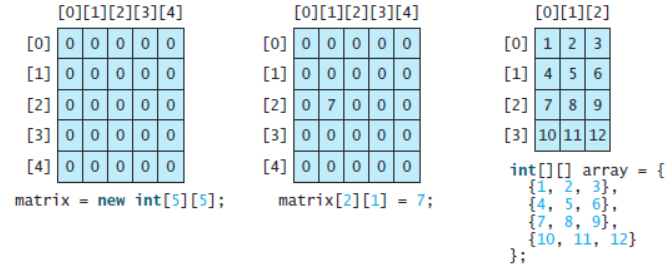
\includegraphics[scale=0.9]{array.png}
	\end{itemize}
\end{itemize}
\newpage
\section{Object Oriented Programming (1)}
\begin{itemize}
	\item Object-Oriented Thinking
	\begin{itemize}
		\item Procedural paradigm
		\begin{itemize}
			\item Focuses on designing methods
			\item Data and operations on the data are separate
		\end{itemize}
		\item Object-oriented paradigm
		\begin{itemize}
			\item Couples methods and data together into objects
			\item Organizes programs in a way that mirrors the real world
			\item A program can be viewed as a collection of cooperating objects
			\item Makes programs easier to develop and maintain
			\item Improves software reusability
		\end{itemize}
	\end{itemize}

	\item Inheritance
	\begin{itemize}
		\item Powerful feature for reusing software
		\item Helps avoid redundancy
		\item Different objects might have common properties and behaviors
		\begin{itemize}
			\item e.g. Person, Employee
		\end{itemize}
		\item Inheritance allows developers to
		\begin{itemize}
			\item Define a general class (or superclass). E.g. Person
			\item Extend the general class to a specialized class (or subclass). e.g. Employee
		\end{itemize}
		\item In Java, the keyword extends is used to indicate inheritance
	\end{itemize}

	\item Casting objects and the \textit{\textbf{instanceof}} operator
	\begin{itemize}
		\item It is always possible to cast an instance of a subclass to a variable of a superclass (known as upcasting)
		\begin{itemize}
			\item e.g. \textbf{Person p = new Employee();}
		\end{itemize}
		\item When casting an instance of a superclass to a variable of its subclass (known as \textit{downcasting}), explicit casting must be used
		\begin{itemize}
			\item e.g. \textbf{Person p = new Employee(); Employee e = (Employee)p;}
			\item If the superclass object is not an instance of the subclass, a runtime error occurs
			\item  It is a good practice to ensure that the object is an instance of another object before attempting a casting. This can be accomplished by using the \textit{\textbf{instanceof}} operator
		\end{itemize}
		\item Cating an object reference does not create a new object
	\end{itemize}

	\item Overloading and Overriding
	\begin{itemize}
		\item Overloading
		\begin{itemize}
			\item Defining methods having the same name but different signatures
			\begin{itemize}
				\item Signature: method name + types of its formal parameters
			\end{itemize}
			\item Overloading methods can make programs clearer and more readable
		\end{itemize}
		\item Overriding
		\begin{itemize}
			\item Defining a method in the subclass using the same signature and the same
			return type as in its superclass
			\item The \textbf{\textit{@Override}} annotation helps avoid mistakes
			\item A static method \textit{cannot} be overridden (it can be invoked using the syntax\\
			SuperClassName.staticMethodName)
		\end{itemize}
	\end{itemize}

	\item The \textbf{\textit{super}} keyword
	\begin{itemize}
		\item Refers to the superclass
		\item Can be used to invoke a superclass constructor
		\begin{itemize}
			\item Syntax: \textbf{\textit{super}}() or \textbf{\textit{super}}(parameters)
			\item  Must be the first statement of the subclass constructor
			\item  A constructor may invoke an overloaded constructor or its superclass constructor. If neither is invoked explicitly, the compiler automatically puts super() as the first statement in the constructor
			\item  If a class is designed to be extended, it is better to provide a no-argument constructor to avoid programming errors
		\end{itemize}
		\item Can be used to invoke a superclass method
		\begin{itemize}
			\item Syntax: \textbf{\textit{super}.methodName}(parameters)
			\item Useful in the case of overridden methods
		\end{itemize}
	\end{itemize}

%	\newpage
	\item The \textbf{\textit{Object}} class
	\begin{itemize}
		\item Every Java class has \textbf{\textit{Object}} as superclass
		\item It has methods that are usually overwritten
		\begin{itemize}
			\item \textbf{\textit{equals}}
			\item \textbf{\textit{hashCode }}
			\item \textbf{\textit{toString}}
		\end{itemize}
		\item \textbf{\textit{equals}} method
		\begin{itemize}
			\item Header: \textbf{\textit{boolean equals(Object obj)}}
			\item The implementation provided by the \textbf{\textit{Object}} class checks whether two reference variables point to the same object
			\begin{itemize}
				\item 	Does not check ``logical equality"
			\end{itemize}
		\end{itemize}
		\item \textbf{\textit{hashCode}} method
		\begin{itemize}
			\item  Header: \textbf{\textit{int hashCode()}}
			\item  The implementation provided by the \textbf{\textit{Object}} class returns the memory address of the object
			\item The \textbf{\textit{hashCode}} method should be overridden in every class that overrides \textbf{\textit{equals}}
			\begin{itemize}
				\item Equal objects must have equal hash codes
			\end{itemize}
			\item A good hashCode method tends to produce unequal hash
			codes for unequal objects
		\end{itemize}
		\item \textbf{\textit{toString}} method
		\begin{itemize}
			\item Header: \textbf{\textit{String toString()}}
			\item The \textbf{\textit{toString}} method is automatically invoked when an object is passed to \textbf{\textit{println}} and the string concatenation operator
			\item Class \textbf{\textit{Object}} provides an implementation of the \textbf{\textit{toString}} method that returns a string consisting of the class name followed by an “at” sign (@) and the unsigned hexadecimal representation of the hash code
			\item \textbf{\textit{toString }}is usually overridden so that it returns a descriptive string representation of the object
		\end{itemize}
	\end{itemize}


	\item Polymorphism
	\begin{itemize}
		\item Every instance of a subclass is also an instance of its superclass, but not vice versa
		\item Polymorphism: An object of a subclass can be used wherever its superclass object is used
		\item Example\\
		\begin{minipage}{0.3\textwidth}
			\centering
			\begin{Verbatim}
	public class Demo {
		public static void main(String [] args) {
			m(new Point(1,2));
		}

		public static void m(Object x) {
			System.out.println(x);
		}
	}
			\end{Verbatim}
		\end{minipage}
	\end{itemize}

	\item Dynamic Binding
	\begin{itemize}
		\item A method can be implemented in several classes along the inheritance chain
		\item The JVM dynamically binds the implementation of the method at runtime, decided by the actual type of the variable
		\begin{itemize}
			\item \textbf{Object x = new Point(1,2);} \hspace{1cm}	//declared type: Object, actual type: Point
		\end{itemize}
		\item Dynamic binding works as follows:
		\begin{itemize}
			\item Suppose an object x is an instance of classes $ C_1, C_2 $, \ldots , $ C_{n-1} $, and $ C_n, $ where $ C_1 $ is a subclass of $ C_2, C_2 $ is a subclass of $ C_3, $ \ldots , and $ C_{n-1} $ is a subclass of $ C_n, $
			\item If x invokes a method p, the JVM searches for the implementation of the method p in $ C_1, C_2, \ldots , C_{n-1}, $ and $ C_n $, in this order, until it is found. Once an implementation is found, the search stops and the first-found implementation is invoked
		\end{itemize}
	\end{itemize}

	\item Encapsulation
	\begin{itemize}
		\item The access control mechanism in Java facilitates encapsulation
		\item There are four possible access levels for members, listed in order of
		increasing accessibility:
		\begin{enumerate}
			\item \textbf{private} -- The member is accessible only from the top-level class where it is declared
			\item \textbf{package-private} -- The member is accessible from any class in the package where it is declared (default access)
			\item \textbf{protected} -- The member is accessible from subclasses of the class where it is declared and from any class in the package where it is declared
			\item \textbf{public} --  the member is accessible from anywhere
		\end{enumerate}
		\item Rule of thumb: \textit{make each member as inaccessible as possible}
	\end{itemize}
\end{itemize}

\newpage
\section{Object Oriented Programming (2)}

\begin{itemize}
	\item Abstract Classes
	\begin{itemize}
		\item Cannot be instantiated using the \textbf{new} operator
		\item Usually contain abstract methods that are implemented in concrete subclasses
		\begin{itemize}
			\item e.g. computeArea() in GeometricObject
		\end{itemize}
		\item Abstract classes and abstract methods are denoted using the
		\textbf{abstract} modifier in the header
		\item A class that contains abstract methods must be defined as abstract
		\item If a subclass of an abstract superclass does not implement all the abstract methods, the subclass must be defined as abstract
	\end{itemize}

	\item Interfaces
	\begin{itemize}
		\item An interface can be used to define common behaviour for classes (including unrelated classes)
		\item Contains only constants and abstract methods
		\item Interfaces are denoted using the \textbf{interface} modifier in the header
		\item Example\\
		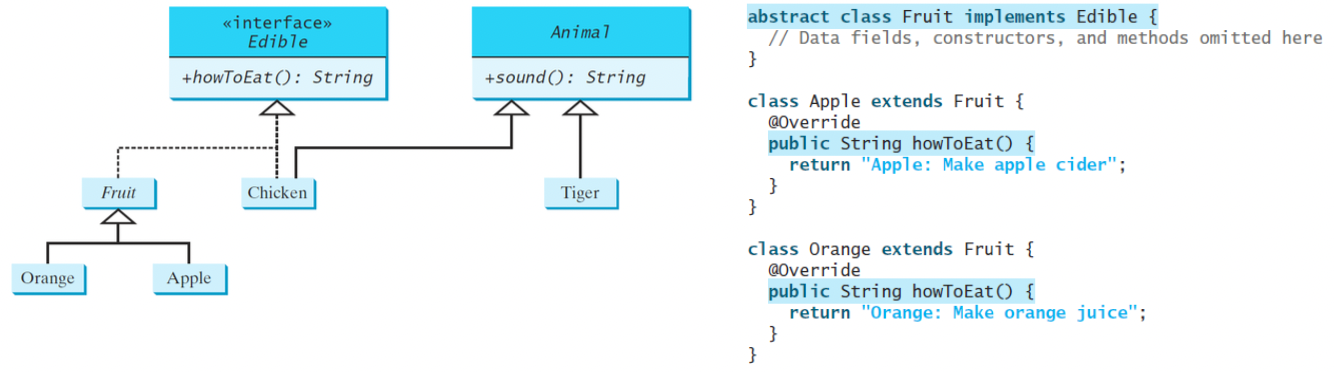
\includegraphics[scale=0.7]{Interface.png}
	\end{itemize}

	\item Generics
	\begin{itemize}
		\item Enable type parameterization
		\begin{itemize}
			\begin{minipage}[h]{\widthof{Generic interfaces} + 1cm}
				\item Generic interfaces
			\end{minipage}
			\begin{minipage}[h]{\widthof{Generic classes} + 1cm}
				\item Generic classes
			\end{minipage}
			\begin{minipage}[h]{\widthof{Generic methods} + 1cm}
				\item Generic methods
			\end{minipage}
		\end{itemize}
		\item Example: \textbf{ArrayList} class
		\begin{itemize}
			\item ArrayList$\langle$Integer$\rangle$ A = new ArrayList$\langle$Integer$\rangle$();
			\item ArrayList$\langle$String$\rangle$ B = new ArrayList$\langle$String$\rangle$();
		\end{itemize}
		\item Generic types must be reference types
		\item Enable error detection at compile time
		\item The \textbf{Comparable} interface
		\begin{itemize}
			\item Defines the \textbf{compareTo} method for comparing objects
			\item Defined as follows:\\[5pt]
			\begin{minipage}{0.5\textwidth}
				\begin{Verbatim}
					public interface Comparable<T> {
						public int compareTo(T t);
					}
				\end{Verbatim}
			\end{minipage}
			\item The \textbf{compareTo} method determines the order of the calling object with \textbf{t} and returns a negative integer, zero, or a positive integer if the calling object is less than, equal to, or greater than \textbf{t}
			\item Many classes implement Comparable (e.g. \textbf{String}, \textbf{Integer})
		\end{itemize}
		%			\newpage
		\item The \textbf{ArrayList} class
		\begin{itemize}
			\item Arrays can be used to store lists of objects. However, once an
			array is created, its size is fixed
			\item Java provides the generic class \textbf{ArrayList} whose size is variable
			\item Imported using: \textbf{import java.util.ArrayList;}
			\item Commonly used methods (\textbf{ArrayList<E>})
			\begin{itemize}
				\item \textbf{boolean add(E e)}
				\item \textbf{E get(int index)}
				\item \textbf{int size()}
				\item \textbf{boolean contains(Object o)}
				\item \textbf{int indexOf(Object o)}
			\end{itemize}
			\item An \textbf{ArrayList} could be traversed using a for-each loop
		\end{itemize}
		%		\newpage
		\item The \textbf{HashSet} class
		\begin{itemize}
			\item Generic class that can be used to store elements without duplicates
			\begin{itemize}
				\item No two elements e1 and e2 can be in the set such that e1.equals(e2) is true
			\end{itemize}
			\item Imported using: \textbf{import java.util.HashSet;}
			\item Objects added to the hash set should override \textbf{equals} and \textbf{hashCode} properly
			\item Commonly used methods (\textbf{HashSet$\langle$E$\rangle$})
			\begin{itemize}
				\item \textbf{boolean add(E e)}
				\item \textbf{int size()}
				\item \textbf{boolean contains(Object o)}
			\end{itemize}
			\item A \textbf{HashSet} could be traversed using a for-each loop
		\end{itemize}

		\item The \textbf{LinkedHashSet} class
		\begin{itemize}
			\item Elements of a \textbf{HashSet} are not necessarily stored in the same
			order they were added
			\item \textbf{LinkedHashSet} is a subclass of \textbf{HashSet} with a linked-list implementation that supports an ordering of the elements in the set
			\item Imported using: \textbf{import java.util.LinkedHashSet;}
		\end{itemize}
	\end{itemize}

	\item Exceptions
	\begin{itemize}
		\item Example\\
		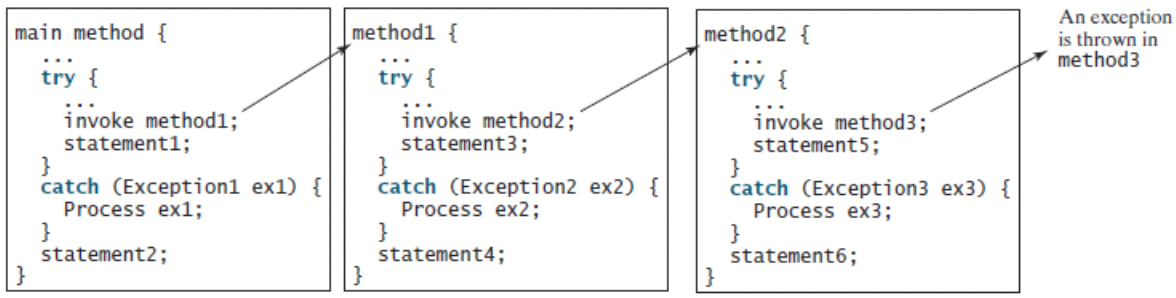
\includegraphics[scale=0.7]{Exceptions.png}
		\item Java has a \textbf{finally} clause that can be used to execute some code regardless of whether an exception occurs or is caught. For example:
		\begin{Verbatim}
			try {
				//statements;
			}
			catch Exception ex) {
				//handling ex; }
			finally {
				//final statements;
			}
		\end{Verbatim}
	\end{itemize}
\end{itemize}
\newpage

\subsection*{Object Oriented Programming - Design Guidelines}
\begin{itemize}
	\item Methods Common to All Objects
	\begin{itemize}
		\item Always override hashCode when you override equals
		\item Always override toString
		\item ConsiderimplementingComparable
	\end{itemize}

	\item Classes and Interfaces
	\vspace{\the\itemsep}
	\begin{itemize}
		 \begin{minipage}[h]{\widthof{Favor composition over inheritance} + 1cm}
			\item Minimize accessibility
			\item Favor composition over inheritance
		\end{minipage}
		\begin{minipage}[h]{\widthof{Prefer interfaces to abstract classes} + 1cm}
			\item Prefer interfaces to abstract classes
			\item Prefer lists to arrays
		\end{minipage}
	\end{itemize}


	\item Methods
	\begin{itemize}
		\item Check parameters for validity
		\item Return empty arrays or collections, not \textbf{null}
		\item Document your API properly
	\end{itemize}

	\item Exceptions
	\begin{itemize}
		\item Use exceptions only for exceptional conditions
		\item Use checked exceptions for recoverable conditions and runtime exceptions for programming errors
		\item Do not ignore exceptions
	\end{itemize}

	\item General Programming (Naming Conventions)
	\begin{itemize}
		\item Package names should be hierarchical with the components separated by periods. Components should consist of lowercase alphabetic characters and, rarely, digits. e.g. \textbf{javax.swing.plaf.metal}
		\item Class and interface names should consist of one or more words, with the first letter of each word capitalized
		\item Method and field names follow the same typographical conventions as class and interface names, except that the first letter of a method or field name should be lowercase, for example, \textbf{ensureCapacity}
		\item The names of constant fields should consist of one or more uppercase words separated by the underscore character, for example, \textbf{NEGATIVE\textunderscore INFINITY}
		\item Local variable names have similar typographical naming conventions to member names, except that abbreviations are permitted, as are individual characters and short sequences of characters whose meaning depends on the context in which the local variable occurs, for example, \textbf{i}, \textbf{xref}
	\end{itemize}
\end{itemize}
\newpage
\section{Software Testing}
\begin{itemize}
	\item What is Software Testing?
	\begin{itemize}
		\item Running a program in order to find faults
		\begin{itemize}
			\item Examining the code without execution is \underline{not} testing
		\end{itemize}
		\item The main practical approach to validate/verify software
		\begin{itemize}
			\item Formal methods that aim at proving the correctness of a program are not
			scalable
		\end{itemize}
		\item “Program testing can be used to show the presence of bugs, but never to show their absence!” -- Edsger W. Dijkstra
	\end{itemize}
	\item Testing Levels
	\begin{itemize}
		\item Acceptance testing
		\begin{itemize}
			\item Test whether the software is acceptable to the user
		\end{itemize}
		\item System testing
		\begin{itemize}
			\item Test the overall functionality of the system
		\end{itemize}
		\item Integration testing
		\begin{itemize}
			\item Test how modules interact with each other
		\end{itemize}
		\item Module testing
		\begin{itemize}
			\item A module is a collection of related units the are assembled in a file, package, or class
			\item Test modules in isolation including how the components interact with each other
			\item \underline{Responsibility of the programmer}
		\end{itemize}
		\item Unit testing
		\begin{itemize}
			\item Test units (methods individually)
			\item \underline{Responsibility of the programmer}
		\end{itemize}
	\end{itemize}

	\item Black-Box and White-Box Testing
	\begin{itemize}
		\item Black-Box Testing
		\begin{itemize}
			\item Test are derived from external descriptions of the software
		\end{itemize}
		\item White-Box Testing
		\begin{itemize}
			\item Test are derived from source code internals of the software
			\item More expensive to apply
		\end{itemize}
	\end{itemize}

	\item Why is Software Testing Hard?
	\begin{itemize}
		\item Exhaustive testing is infeasible
		\begin{itemize}
			\item e.g. Exhaustively testing a method with two integer parameters would
			require $ \sim \negmedspace 10^{19} $ tests
		\end{itemize}
		\item Random/statistical testing is not effective
	\end{itemize}

	\item Why Do We Test Software?
	\begin{itemize}
		\item Software is everywhere
		\begin{itemize}
			\item Communication, transportation, healthcare, finance, education, etc.
		\end{itemize}
		\item Software failures could have severe consequences
		\begin{itemize}
			\item A 2002 NIST report estimated that defective software costs the U.S. economy \$59.5 billion per year and that improvements in testing could reduce this cost by about a third
			\item In certain areas such as healthcare and transportation, software failures could cost lives
		\end{itemize}
	\end{itemize}

	\item Infamous Software Failures
	\begin{itemize}
		\item Northeast blackout of 2003
		\begin{itemize}
			\item Caused by a failure of the alarm system
			\item Affected 40 million people in USA and 10 million people in Canada
			\item Contributed to at least 11 deaths
			\item Cost around \$6 billion
		\end{itemize}
		\item Ariane 5 explosion (1996)
		\begin{itemize}
			\item Unhandled floating point conversion exception
			\item Estimated loss: \$370 million
		\end{itemize}
		\item NASA’s Mars lander (1999)
		\begin{itemize}
			\item Crashed due to an integration fault
			\item Estimated loss: \$165 million
		\end{itemize}
		\item Boeing 737 Max
		\begin{itemize}
			\item Crashed due to overly aggressive software flight overrides
		\end{itemize}
		\item Boeing A220
		\begin{itemize}
			\item Engines failed after software update allowed excessive vibrations
		\end{itemize}
		\item Toyota brakes failure
		\begin{itemize}
			\item Dozens dead
			\item Thousands of crashes
		\end{itemize}
		\item Therac-25 radiation therapy machine
		\begin{itemize}
			\item Three patients were killed
		\end{itemize}
	\end{itemize}

	\item Fault/Error/Failure
	\begin{itemize}
		\item \textbf{\textit{Software Fault}}: A static defect in the software
		\item \textbf{\textit{Software Error}}: An incorrect internal state that is the manifestation of
		some fault
		\item \textbf{\textit{Software Failure}}: External, incorrect behavior with respect to the requirements or another description of the expected behaviour
		\item The term \textbf{\textit{bug }}is often used informally to refer to all three of fault, error, and failure
		\begin{itemize}
			\item The first computer bug was an actual bug!
		\end{itemize}
		\item Example\\
		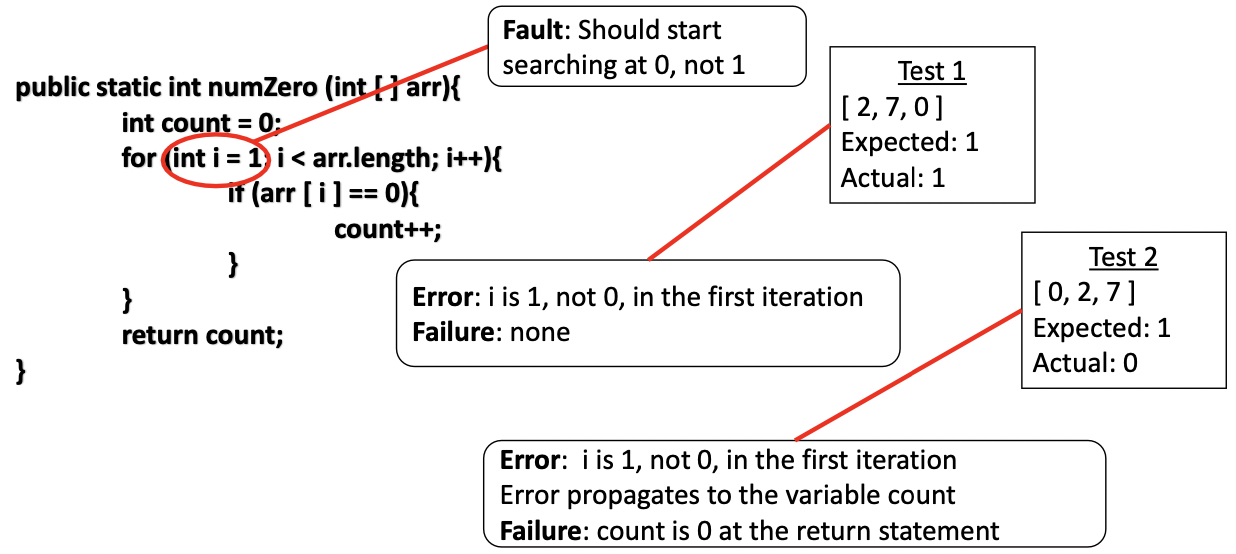
\includegraphics[scale=0.7]{FEF.png}
	\end{itemize}

	\newpage
	\item The RIPR model
	\begin{itemize}
		\item Four conditions are needed for a failure to be observed
		\begin{enumerate}
			\item \textbf{\textit{Reachability}}: a test must reach the location in the program that contains the fault
			\item \textbf{\textit{Infection}}: After the faulty location is executed, the state of the program must be incorrect
			\item \textbf{\textit{Propagation}}: The infected state must propagate through the rest of the execution and cause some output or final state of the program to be incorrect
			\item \textbf{\textit{Revealability}}: The tester must observe part of the incorrect portion of the final program state
		\end{enumerate}
		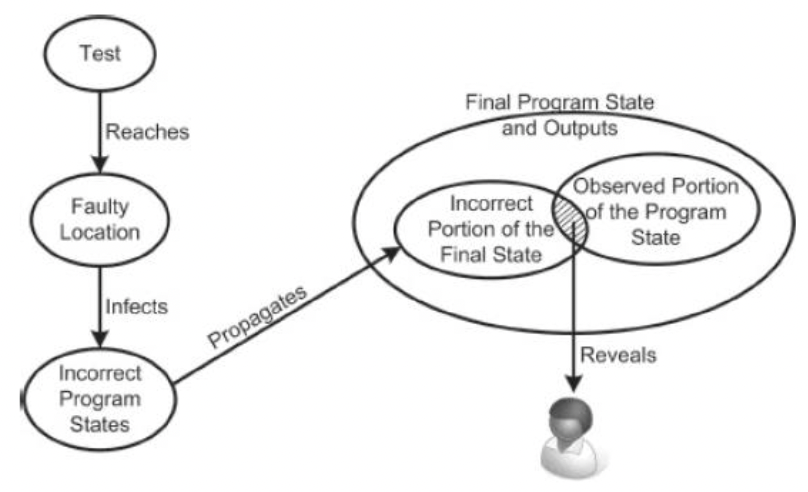
\includegraphics[scale=0.7]{RIPR.png}
	\end{itemize}

	\item Criteria-based Test Design
	\begin{itemize}
		\item \textbf{\textit{Coverage Criterion}}: A rule or collection of rules that impose test requirements on a test set
		\begin{itemize}
			\item e.g. For each statement in the code, there should be at least one test case that covers it
		\end{itemize}
		\item Coverage criteria give us structured, practical ways to search the input space. Satisfying a coverage criterion gives a tester some amount of confidence in two crucial goals:
		\begin{enumerate}
			\item We have looked in many corners of the input space, and
			\item Our tests have a fairly low amount of overlap
		\end{enumerate}
		\item Criteria subsumption
		\begin{itemize}
			\item $ C_1 $ subsumes $ C_2 $ if and only if every test set that satisfies $ C_1 $ satisfies $ C_2 $
		\end{itemize}
	\end{itemize}

	\item Graph Coverage
	\begin{itemize}
		\item The software is modeled as a graph where nodes and edges could represent:
		\begin{itemize}
			\item Methods and calls
			\item Statements and branches
			\item Etc.
		\end{itemize}
		\item Coverage criteria are defined based on the graph. For example:
		\begin{itemize}
			\item Cover every node
			\item Cover every edge
			\item Cover every path
			\item Etc.
		\end{itemize}


		\item Example (Control Flow Graph)\\
		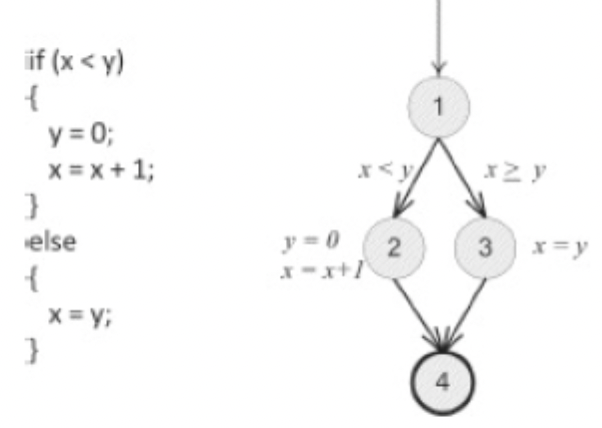
\includegraphics[scale=0.7]{CFG.png}
	\end{itemize}

	\item Logic Coverage
	\begin{itemize}
		\item Involves the boolean expressions of the code
		\item Coverage criteria include:
		\begin{itemize}
			\item Predicate coverage
			\item Clause coverage
			\item Combinational coverage
			\item Etc.
		\end{itemize}
		\item Example
		\begin{Verbatim}
			if(((a>b) || c) && (x<y))
			...
			else
			...
		\end{Verbatim}
		\item Predicate coverage
		\begin{itemize}
			\item The test set should make each predicate evaluate to true and false
			\item e.g. $ ((a>b) \, || \, c) \, \&\& \, (x<y) = \{\text{True}, \text{False}\} $
		\end{itemize}
		\item Clause coverage
		\begin{itemize}
			\item The test set should make each clause evaluate to true and false
			\item e.g. $ (a>b) = \{\text{True}, \text{False}\}, c = \{\text{True}, \text{False}\}, (x<y) = \{\text{True}, \text{False}\} $
		\end{itemize}
	\end{itemize}

	\item Active clause coverage
	\begin{itemize}
		\item Clause coverage has a weakness
		\begin{itemize}
			\item The values do not always make a difference
		\end{itemize}
		\item A clause $ c_i$ in predicate $ p $, called the major clause, determines $ p $ \textit{if and only if} the values of the remaining minor clauses $ c_j $ are such that changing $ c_i $ changes the value of $ p $
		\item Two requirements for each $ c_i $: $ c_i $ evaluates to true and $ c_i $ evaluates to false
		\item This is a form of MCDC, which is required by the FAA for safety critical
		software

	\end{itemize}

	\item Inactive clause coverage
	\begin{itemize}
		\item Ensures that “major” clauses do not affect the predicates
		\item Four requirements for each $ c_i $
		\begin{enumerate}
			\item $c_i$ evaluates to true with p true
			\item $c_i$ evaluates to false with p true
			\item $c_i$ evaluates to true with p false
			\item $c_i$ evaluates to false with p false
		\end{enumerate}
		\item Example
		\begin{itemize}
			\item Testing the control software for a shutdown system in a reactor where the specification states that the status of a particular valve (\textbf{open} vs. \textbf{closed}) is relevant to the reset operation in \textbf{Normal} mode, but not in \textbf{Override} mode
		\end{itemize}
	\end{itemize}

	\item Test Oracles
	\begin{itemize}
		\item A \textit{test oracle} is an encoding of the expected results of a given test
		\begin{itemize}
			\item e.g. JUnit assertion
		\end{itemize}
		\item Must strike a balance between checking too much (unnecessary cost) and checking too little (perhaps not revealing failures)
		\item What should be checked?
		\begin{itemize}
			\item The output state is everything that is produced by the software under test, including outputs to the screen, file, databases, messages, and signals
			\item Each test should have a goal and testers should check the output(s) that are mainly related to that goal
			\begin{itemize}
				\item At the unit testing level, checking the return values of the methods and returned parameter values are almost always enough
				\item At the system level, it is usually sufficient to check the directly visible output such as to the screen
			\end{itemize}
		\end{itemize}

		\item How to determine what the correct results are
		\begin{itemize}
			\item Specification-Based direct verification of outputs
			\begin{itemize}
				\item e.g. “a \textbf{sort} program should produce a permutation of its input in increasing order ”
				\item Specifications are hard to write
			\end{itemize}
			\item Redundant computations
			\begin{itemize}
				\item Refer to another trustworthy implementation of the program
				\item Usually used for regression testing
			\end{itemize}
			\item Consistency checks
			\begin{itemize}
				\item Check whether certain properties hold (e.g. a value representing probability
				should neither be negative nor larger than one)
			\end{itemize}
		\end{itemize}
	\end{itemize}
\end{itemize}

\newpage
\section{Design Patterns}
\begin{itemize}
	\item What are Design Patterns
	\begin{itemize}
		\item Descriptions of communicating objects and classes that are customized to \textbf{\underline{solve}} a general design \textbf{\underline{problem}} in a particular \textbf{\underline{context}}
		\item 	Gamma et al. described 23 design patterns divided into three categories:
		\begin{enumerate}
			\item Creational patterns
			\item Structural patterns
			\item Behavioral patterns
		\end{enumerate}
	\end{itemize}

	\item Creational Patterns
	\begin{itemize}
		\item Concern the process of object creation
		\item Six creational patterns
		\vspace{-\itemsep}
		\begin{enumerate}
		\begin{minipage}[t]{\widthof{Abstract Factory} + 1cm}
%			\begin{enumerate}
				\item Factory Method
				\item Abstract Factory
				\item Singleton
%			\end{enumerate}
		\end{minipage}
		\begin{minipage}[t]{\widthof{Object pool} + 1cm}
%			\begin{enumerate}
				\setcounter{enumi}{3}
				\item Prototype
				\item Builder
				\item Object Pool
%			\end{enumerate}
		\end{minipage}
		\end{enumerate}
	\end{itemize}

	\item Structural Patterns
	\begin{itemize}
		\item Deal with the composition of classes or objects
		\item Seven structural patterns
		\vspace{-\itemsep}
		\begin{enumerate}
		\begin{minipage}[t]{\widthof{Composite} + 1cm}
				\item Adapter
				\item Bridge
				\item Composite
				\item Decorator
		\end{minipage}
		\begin{minipage}[t]{\widthof{Flyweight} + 1cm}
				\setcounter{enumi}{4}
				\item Facade
				\item Flyweight
				\item Proxy
		\end{minipage}
		\end{enumerate}
	\end{itemize}

	\item Behavioral Patterns
	\begin{itemize}
		\item Characterize the ways in which classes or objects interact and distribute responsibility
		\item Ten Behavioral patterns
		\begin{enumerate}
		\begin{minipage}[t]{\widthof{Chain of Responsibility} + 1cm}
				\item Chain of Responsibility
				\item Command
				\item Interpreter
				\item Iterator
				\item Mediator
		\end{minipage}
		\begin{minipage}[t]{\widthof{Observer} + 1cm}
				\setcounter{enumi}{5}
				\item Memento
				\item Observer
				\item State
				\item Strategy
				\item Template
		\end{minipage}
		\end{enumerate}
	\end{itemize}

	\item Singleton (Creational)
	\begin{itemize}
		\item Intent: Ensure a class has only one instance, and provide a global point of access to it\\
		\begin{center}
			\begin{tabular}{| l |}
				\hline
				Singleton\\
				\hline
				$ - $instance: Singleton\\
				\hline
				$ - $Singleton()\\
				+getInstance(): Singleton\\
				\ldots\\
				\hline
			\end{tabular}	\textit{	( $ - $ means private, $ + $ means public)}
		\end{center}
	\end{itemize}
	%
	\item Facade (Structural)
	\begin{itemize}
		\item Intent: Hide complexities and provide a unified interface to a set of interfaces in a subsystem\\[-10pt]
		\begin{center}
			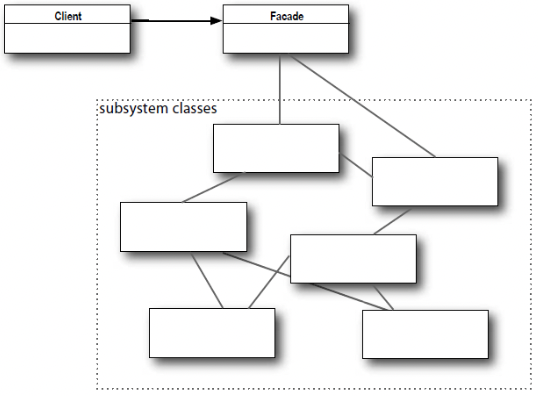
\includegraphics[scale=0.8]{Facad.png}
		\end{center}
	\end{itemize}
%	\newpage
	\item Adapter (Structural)
	\begin{itemize}
		\item Intent: Let classes work together that couldn't otherwise because of incompatible interfaces\\[-10pt]
		\begin{center}
			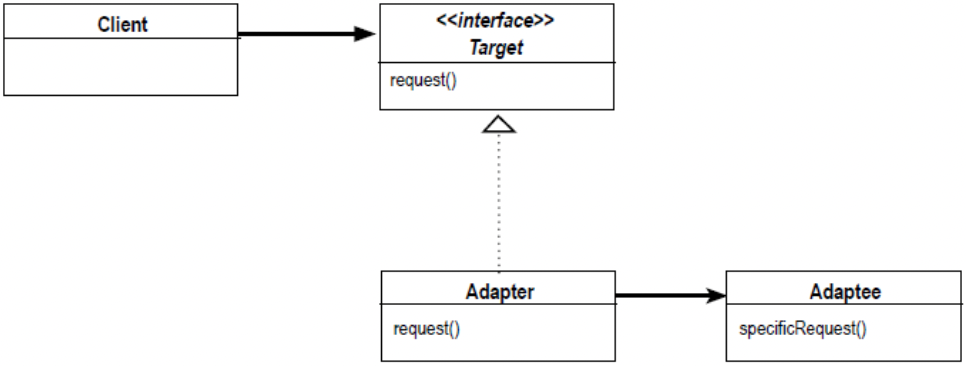
\includegraphics[scale=0.7]{Adapter.png}
		\end{center}
	\end{itemize}

	\item Observer (Behavioral)
	\begin{itemize}
		\item Intent: Define a one-to-many dependency between objects so that when one object changes state, all its dependents are notified and updated automatically\\[-10pt]
		\begin{center}
			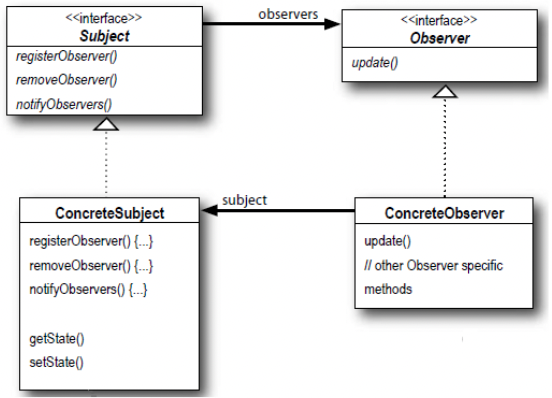
\includegraphics[scale=0.9]{Observer.png}
		\end{center}
	\end{itemize}
	%	\newpage
	\item Strategy (Behavioral)
	\begin{itemize}
		\item Intent: Define a family of algorithms, encapsulate each one, and make them interchangeable\\[-10pt]
		\begin{center}
			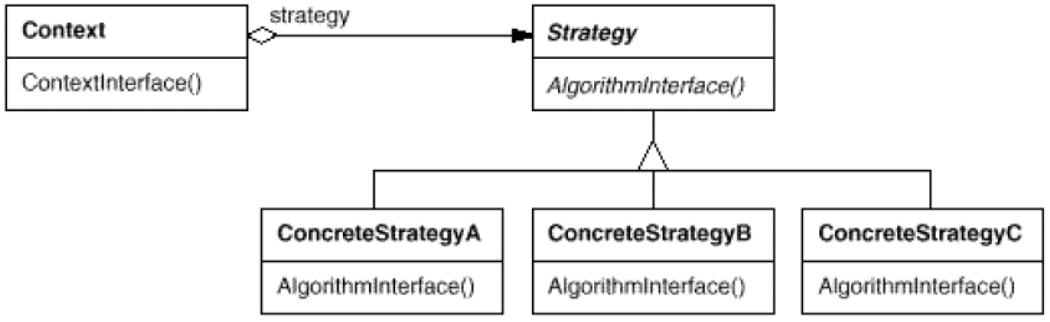
\includegraphics[scale=0.8]{Strategy.png}
		\end{center}
	\end{itemize}
\end{itemize}

\newpage
%\input{preamble.txt}
%
%\begin{document}
\section{SOLID Design}

\begin{itemize}
	\item What is SOLID?
	\begin{itemize}
		\item \textbf{S}ingle Responsibility Principle
		\item \textbf{O}pen/Closed Principle
		\item \textbf{L}iskov Substitution Principle
		\item \textbf{I}nterface Segregation Principle
		\item \textbf{D}ependency Inversion Principle
	\end{itemize}

	\item Single Responsibility Principle (SRP)\\
	\textbf{\emph{A class should have only one reason to change}}
	\begin{itemize}
		\item If you can think of more than one motive for changing a class, then that class has more than one responsibility
		\item If a class has more than one responsibility, then the responsibilities become coupled
		\item Violating the SRP\\
		\begin{center}
			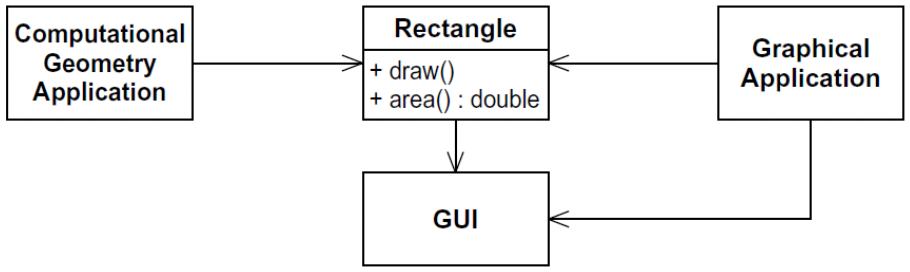
\includegraphics[width=0.6\linewidth]{SRPViolation}
		\end{center}
		\item Conforming to the SRP
		\begin{center}
			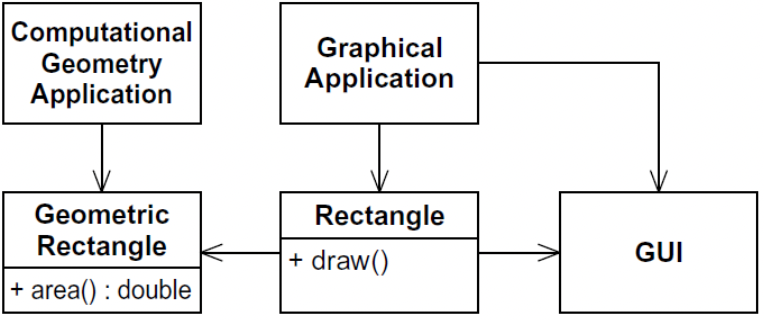
\includegraphics[width=0.5\linewidth]{SRPConform}
		\end{center}
	\end{itemize}

	\item The Open/Closed Principle (OCP)\\
	\textbf{\emph{Software entities (classes, modules, functions, etc.) should be open for extension, but closed for modification.}}
	\begin{itemize}
		\item When a single change to a program results in a cascade of changes to dependent modules, the design smells of rigidity.
		\begin{itemize}
			\item If the Open/Closed principle is applied well, then further changes of that kind are achieved by adding new code, not by changing old code that already works.
		\end{itemize}
		\item In Java, it is possible to create abstractions that are fixed and yet represent an unbounded group of possible behaviors
		\begin{itemize}
			\item The abstractions are abstract base classes, and the unbounded group of possible behaviors is represented by all the possible derivative classes.
		\end{itemize}
		\item Violating the OCP
		\begin{itemize}
			\begin{minipage}{0.5\textwidth}
				\item Both classes are concrete
				\item The \textbf{Client} uses the \textbf{Server} class
			\end{minipage}
			\begin{minipage}{0.5\textwidth}
				
\includegraphics[width=1.5in]{OCPViolate}
			\end{minipage}
		\end{itemize}

		\begin{minipage}{0.5\textwidth}
			\item Conforming to the OCP\\
		\end{minipage}
		\begin{minipage}{0.5\textwidth}
			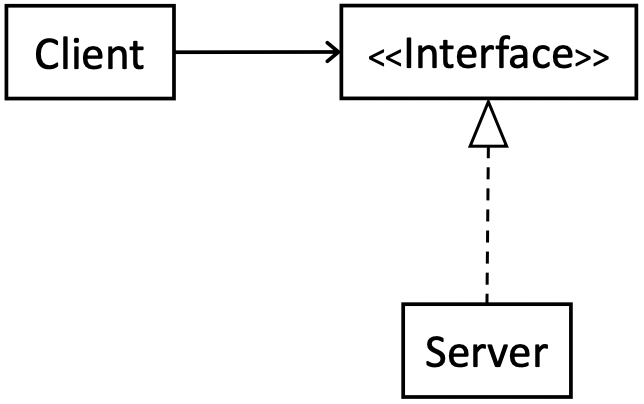
\includegraphics[width=0.4\textwidth]{OCPConform}
		\end{minipage}
	\end{itemize}

	\item The Liskov Substitution Principle (LSP)\\
	\textbf{\emph{Subtypes must be substitutable for their base types.}}
	\begin{itemize}
		\item Formally: Let $ \Phi(x) $ be a property provable about objects $ x $ of type $ T $. Then $ \Phi(y) $ should be true for objects $ y $ of type $ S $ where $ S $ is a subtype of $ T $.
		\item Counter-example: ``If it looks like a duck, quacks like a duck, but needs batteries – you probably have the wrong abstraction"
		\item Violating the LSP\\
		Issues\\
		\begin{minipage}{0.6\textwidth}
			\begin{itemize}
				\item Inheriting \textbf{height} and \textbf{width}
				\item Overriding \textbf{setHeight} and \textbf{setWidth}
				\item Conflicting assumptions. For example:
				\begin{Verbatim}
					void testRectangleArea(Rectangle r){
						r.setWidth(5);
						r.setHeight(4);
						assertEquals(r.computeArea(), 20);
					}
				\end{Verbatim}
			\end{itemize}
		\end{minipage}
		\begin{minipage}{0.3\textwidth}
			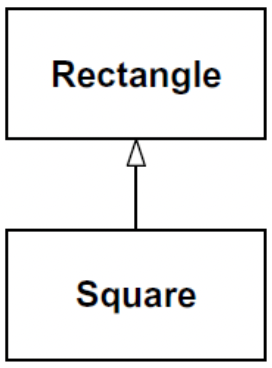
\includegraphics[width=1in]{LSPExample}
		\end{minipage}

		\item Implication: A model, viewed in isolation, cannot be meaningfully validated.
		\begin{itemize}
			\item The validity of a model can only be expressed in terms of its clients.
			\item One must view the design in terms of the reasonable assumptions made by
			the users of that design.
		\end{itemize}
	\end{itemize}

	\item The Interface Segregation Principle (ISP)\\
	\textbf{\emph{Clients should not be forced to depend on methods that they do not use.}}
	\begin{itemize}
		\item This principle deals with classes whose interfaces are not cohesive. That is, the interfaces of the class can be broken up into groups of methods where each group serves a different set of clients.
		\item When clients are forced to depend on methods that they don’t use, then those clients are subject to changes to those methods.\\
		\begin{minipage}[t]{0.4\textwidth}
			\item Violating the ISP\\
			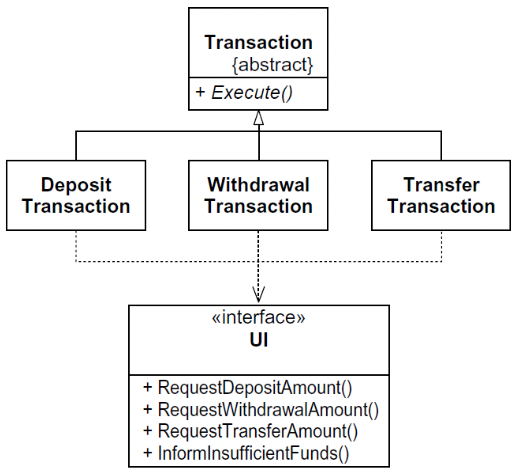
\includegraphics[width=2.5in]{ISPViolation}
		\end{minipage}
		\begin{minipage}[t]{0.6\textwidth}
			\item Conforming to the ISP\\
			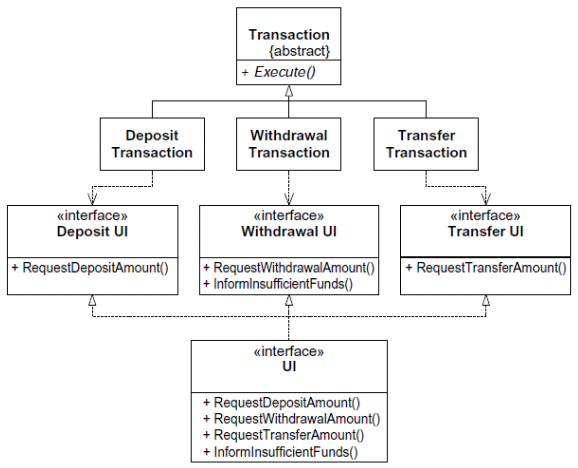
\includegraphics[width=3.5in]{ISPObey}
		\end{minipage}
	\end{itemize}

	\newpage

	\item The Dependency-Inversion Principle (DIP)
	\begin{enumerate}
		\item[\textbf{\textit{A.}}]  \textbf{\textit{High-level modules should not depend on low-level modules. Both should depend on abstractions.}}
		\item[\textbf{\textit{B.}}] \textbf{\textit{Abstractions should not depend on details. Details should depend on abstractions.}}
	\end{enumerate}
	\begin{itemize}
		\item The modules that contain the high-level business rules should take precedence over, and be independent of, the modules that contain the implementation details.
		\item When high-level modules depend on low-level modules, it becomes very difficult to reuse those high-level modules in different contexts.\\
		\begin{minipage}[t]{0.3\textwidth}
			\begin{center}
				\underline{\textbf{Naïve Layering}}\\
				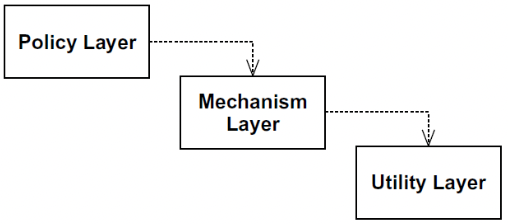
\includegraphics[width=2in]{DIPNaive}
			\end{center}
		\end{minipage}
		\begin{minipage}[t]{0.5\textwidth}
			\begin{center}
				\underline{\textbf{Inverted Layers}}\\
				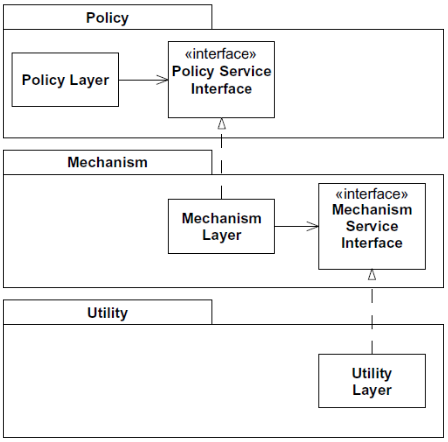
\includegraphics[width=2.5in]{DIPInverted}
			\end{center}
		\end{minipage}
		\\[10pt]
		\begin{minipage}[t]{0.5\textwidth}
			\item Violating the DIP\\
			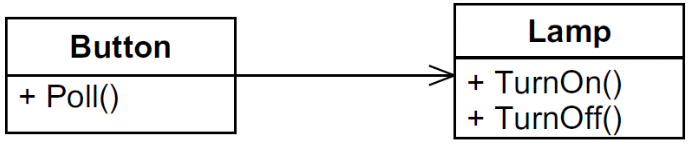
\includegraphics[width=2in]{DIPViolate}
		\end{minipage}
		\begin{minipage}[t]{0.5\textwidth}
			\item Conforming to the DIP\\
			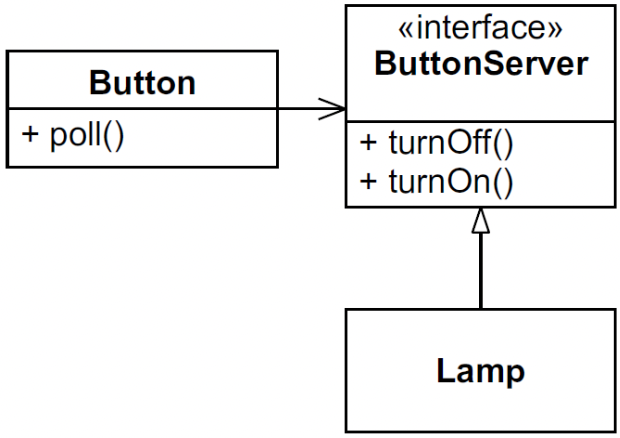
\includegraphics[width=2in]{DIPConform}
		\end{minipage}
	\end{itemize}

	\item Design Smells
	\begin{itemize}
		\item Symptoms of poor design
		\item Often caused by the violation of one or more of the design principles
		\begin{itemize}
			\item For example, the smell of \textit{Rigidity} is often a result of insufficient attention to OCP.
		\end{itemize}
		\item These symptoms include:
		\begin{enumerate}
			\item Rigidity -- The design is hard to change.
			\item Fragility -- The design is easy to break.
			\item Immobility -- The design is hard to reuse.
			\item Viscosity -- It is hard to do the right thing.
			\item Needless Complexity -- Overdesign.
			\item Needless Repetition -- Mouse abuse.
			\item Opacity -- Disorganized expression.
		\end{enumerate}
	\end{itemize}
\end{itemize}

%\end{document}
\newpage
%\input{preamble.txt}

%\begin{document}
\section{Software Development Life Cycle}
\begin{itemize}
	\begin{minipage}{0.65\textwidth}
		\item Software Development Life Cycle (SDLC)
		\begin{itemize}
			\item \textbf{Planning} -- develop a plan for creating the concept or evolution of the concept
			\item \textbf{Analysis} -- analyze the needs of those using the system. Create detailed requirements
			\item \textbf{Design} -- Translate the detailed requirements into detailed design work
			\item \textbf{Implementation} -- Complete the work of developing and testing the system
			\item \textbf{Maintenance} -- Complete any required maintenance to keep the system running
		\end{itemize}
	\end{minipage}
	\begin{minipage}{0.02\textwidth}
	\end{minipage}
	\begin{minipage}{0.33\textwidth}
		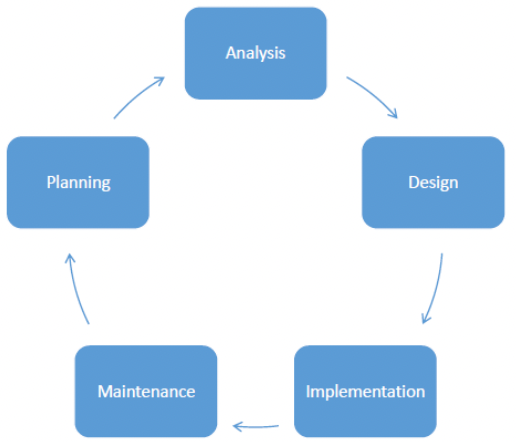
\includegraphics[scale=0.7]{SDLCCircle}
	\end{minipage}

	\item Different SDLC implementations
	\begin{itemize}
		\item Rigid timeline / budget (Waterfall)
		\item Rick Adverse (Spiral)
		\item Quality Deliverables / Less management (Agile)
	\end{itemize}

	\item Waterfall
	\begin{itemize}
		\item A sequential (non-iterative) model
		\item Involves a large amount of upfront work, in an attempt to
		reduce the amount of work done in later phases of the project
	\end{itemize}
	\begin{center}
		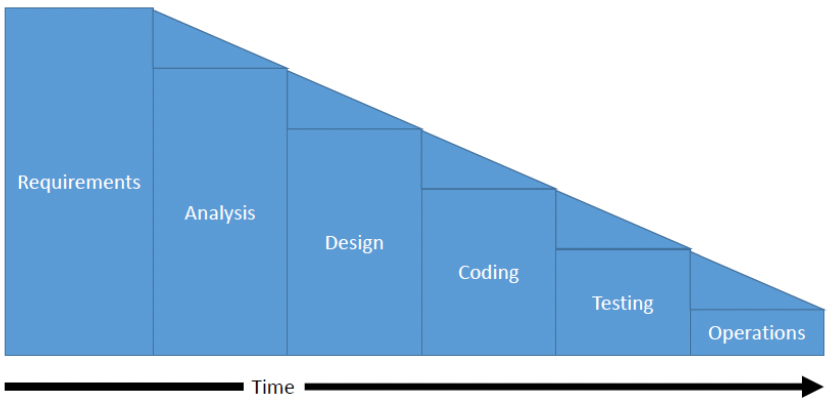
\includegraphics[scale=0.5]{Waterfall}
	\end{center}

	\item Spiral\\
	\begin{minipage}{0.7\textwidth}
		\begin{itemize}
			\item Risk-driven model
			\item More time is spent on a given phase based on the amount of risk that phase poses for the project
		\end{itemize}
	\end{minipage}
	\begin{minipage}{0.3\textwidth}
		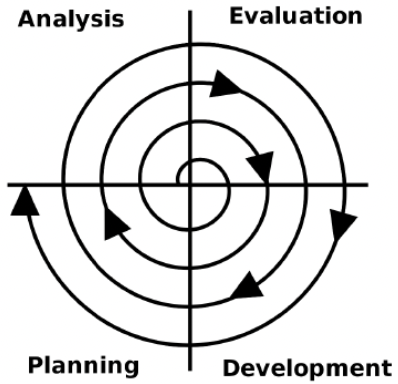
\includegraphics[scale=0.5]{Spiral}
	\end{minipage}

	\item Agile
	\begin{itemize}
		\item Issues with Waterfall
		\begin{itemize}
			\item Inappropriate when requirements change frequently
			\item Time gets squeezed the further into the process you get
		\end{itemize}
		\item Agile Methodologies
		\begin{itemize}
			\item Extreme Programming (XP)
			\item Scrum
			\item Test-driven Develpoment (TDD)
			\item Feature-driven Development (FDD)
			\item Etc.
		\end{itemize}
	\end{itemize}

	\item Agile Manifesto\\
	\emph{``We are uncovering better ways of developing software by doing it and helping others do it. Through this work, we have come to value:\\
		\hspace*{10mm} \textbf{Individuals and interactions} over processes and tools\\
		\hspace*{10mm} \textbf{Working software} over comprehensive documentation\\
		\hspace*{10mm} \textbf{Customer collaboration} over contract negotiation\\
		\hspace*{10mm} \textbf{Reponding to change} over following a plan\\
		That is, while there is value in the items on the right, we value the items on the left more."}

	\item Agile vs. Waterfall\\
		\begin{table}[h]
			\centering
		\begin{tabular}{| r | c c |}
			\hline
			& \textbf{Agile} & \textbf{Waterfall}\\
			\cline{2-3}%
			Iterative? & \cellcolor{green!25}Yes & \cellcolor{green!15}No\\
			Late changes? & \cellcolor{green!25}Yes & \cellcolor{green!15}No / \$\$\$\\
			Fixed timeline? & \cellcolor{green!15}No* & \cellcolor{green!25}Yes\\
			Fixed cost? & \cellcolor{green!15}No* & \cellcolor{green!25}Yes*\\
			Volume of meetings & \cellcolor{green!25}Consistent & Heavy up front, reduced middle, heavy end\\
			Release frequency & \cellcolor{green!25}Every sprint & \cellcolor{green!15}Once per project\\
			Business Involvement & Heavy throughout & Heavy early, and at very end\\
			Cost to fix mistakes & \cellcolor{green!25}Low & \cellcolor{green!15}High\\
			\hline
		\end{tabular}
		\end{table}

	\item eXtreme Programming (XP)
	\begin{itemize}
		\item One of the most rigorous forms of Agile
		\item Involves building a series of feedback loops, which are used to help guide when change can occur and allow for changes to be quickly integrated into the plan for development
		\item Built on the idea that you can reduce the cost of developing software, and build better software, by having goals
		\item XP requires that everything that can be unit tested is unit tested, that everyone works in pairs, and that these pairs change frequently
	\end{itemize}

	\item Code Review
	\begin{itemize}
		\item Although pair programming has gone out of vogue along with XP, it is important to note a practice that has become common place that was born from this idea -- Code Review.
		\item A code review is a session in which you \textbf{must sit down with another developer} from the team and walk them through your implementation line-by-line in order to get advice and feedback.
		\item This process has been shown to lead to better code, through finding bugs earlier, and an increased amount of collaboration on difficult concepts.
	\end{itemize}

	\item Scrum
	\begin{itemize}
		\item Scrum is currently one of the most widely used methodologies of software development\\[-15pt]
	\end{itemize}
	\begin{center}
		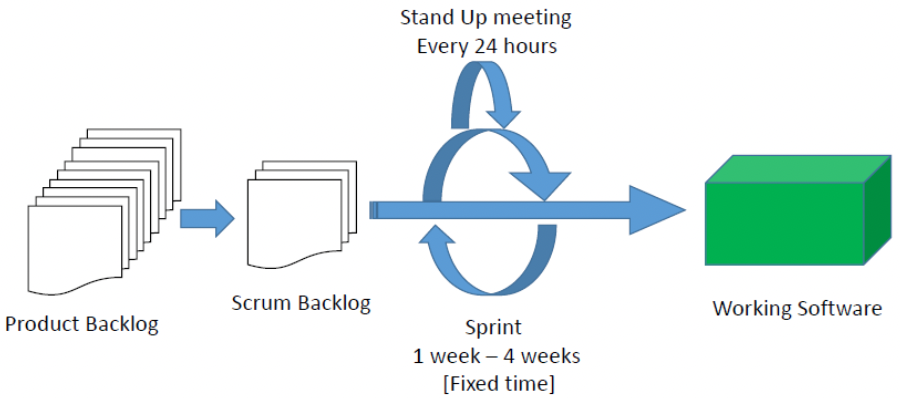
\includegraphics[scale=0.5]{Scrum}
	\end{center}

	\item Scrum - Roles
	\begin{itemize}
		\item Product Owner
		\begin{itemize}
			\item Responsible for delivering requirements and accepting demos
			\item Involved in planning session
		\end{itemize}
		\item Scrum Master
		\begin{itemize}
			\item Responsible for removing impediments
		\end{itemize}
		\item Team members
		\begin{itemize}
			\item No one has a fixed role other than the scrum master and product owner
			\item Everyone takes on tasks, and completes them based on what they are most comfortable with
		\end{itemize}
	\end{itemize}

	\item Scrum - Sprint
	\begin{itemize}
		\item The sprint is a fixed time to deliver a working set of features, that are reviewed in a demonstration to the product owner
		\item Tasks in Scrum are broken into “User Stories”
		\item In a sprint, a team agrees at the beginning to take on a certain
		number of user stories
		\item Sprints are usually between 1 and 4 weeks in length
		\item At the end of each sprint, teams hold a “retrospective” which is a meeting where the past sprint is discussed, and chances for improvement for the next sprint are raised
	\end{itemize}

	\item Scrum - User Stories
	\begin{itemize}
		\item User stories are similar to requirements. They are written in the following format:\\
		\hspace*{10mm}\emph{As a \{ACTOR/OBJECT\} I want to \{ACTION\} so that \{RESULT\}}
	\end{itemize}

	\item Scrum - Planning Poker
	\begin{itemize}
		\item In scrum, we do not assign time to tasks, but assign arbitrary points. This is a form of estimation that helps gauge how much work something will take to complete.
		\item Planning poker takes a set of pre-determined numbers (usually: 1, 2, 3, 5, 8, etc.) and gets you to estimate how much work something will be relative to a known task.
		\item After discussing the story at hand , everyone selects a card. Then, the cards are turned over simultaneously. Usually time is given for those who had the lowest and highest numbers to state their case
		\item The process is repeated until everyone ends up at the same number.
	\end{itemize}

	\item Scrum - Planning Session
	\begin{itemize}
		\item Planning sessions happen at the start of each sprint.
		\item They usually take a few hours. During this time, the team decides how much work it will take on, and discusses any major technical challenges they expect to face.
		\item Usually, Product Owners are available for at least a portion of this meeting, to help with prioritization. They are only there to assist in this regard, and not to dictate what the team will complete.
	\end{itemize}

	\item Scrum - The Standup Meeting
	\begin{itemize}
		\item Happens EVERY SINGLE day that you are working
		\item The goal is to make sure people are doing alright
		\item Shouldn’t be longer than 15 minutes
		\item Answer three questions:
		\begin{enumerate}
			\item What did I finish since the last standup?
			\item What am I going to finish by the next standup?
			\item What is stopping me / what impediments am I facing?
		\end{enumerate}
	\end{itemize}

	\item Scrum - Working Agreement
	\begin{itemize}
		\item A series of statements that everyone on the team agrees to about how the team will work
		\item Things in working agreements may include:
		\begin{itemize}
			\item The standup will occur at 1:00 pm every day, and last 15 minutes
			\item We will not speak during the standup, unless it is our turn to speak
			\item Our meetings will take place in the lobby of the IC building
			\item All code must be peer-reviewed
			\item We will submit all code 24 hours prior to the due date
		\end{itemize}
	\end{itemize}

	\item Scrum - Definition of Done
	\begin{itemize}
		\item A formal agreement of when work is considered complete
		\item For example, a story can be marked as done when:
		\begin{itemize}
			\item It has been fully unit tested
			\item It successfully integrated with the rest of the code
			\item It has been peer reviewed
			\item It is fully commented
			\item Etc.
		\end{itemize}
		\item It is important that team comes to an agreement on this definition before they start work.
	\end{itemize}

	\item Test Driven Development (TDD)
	\begin{itemize}
		\item TDD is a way to develop software that revolves around writing test cases.
		\item The basic concept is to write the unit tests needed to be passed for a feature to be considered working. You then code to the unit tests –writing the minimum amount for the tests to succeed.
		\item Once working, you review and refactor. Then move on to the next set of tests.\\[-15pt]
		\begin{center}
			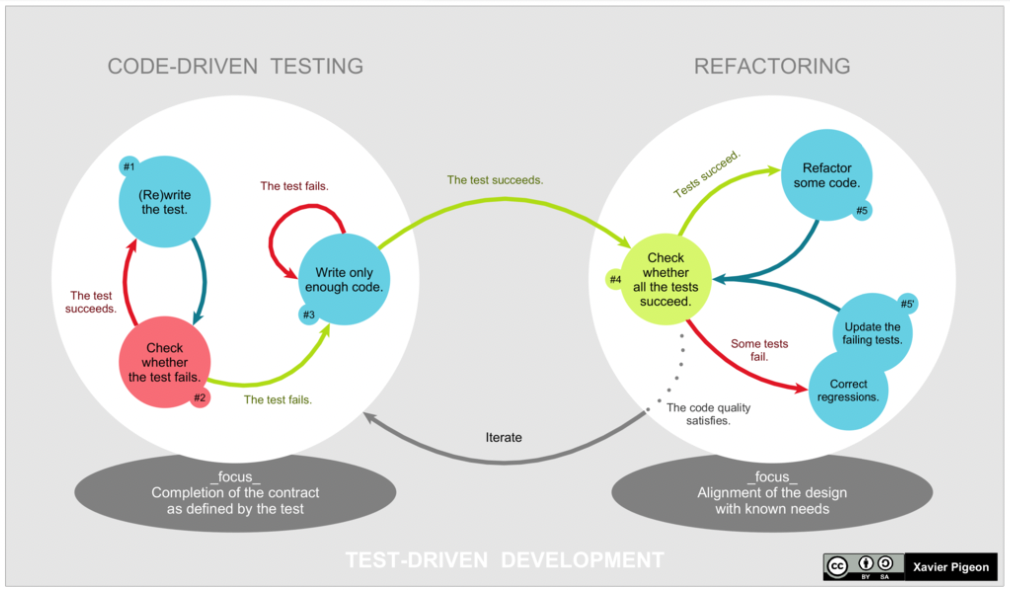
\includegraphics[scale=0.8]{TDD}
		\end{center}
	\end{itemize}

	\item Feature Driven Development (FDD)
	\begin{itemize}
		\item Based on the idea of building a focused model for the project, and the iterating on the features needed.
		\item Splits development into 5 major pieces:
		\begin{enumerate}
			\item Develop overall model
			\item Build feature list
			\item Plan by feature
			\item Design by feature
			\item Build by feature
		\end{enumerate}
	\end{itemize}

\end{itemize}

%\end{document}
\newpage
%\input{preamble.txt}
%
%\begin{document}
\section{I/O and Regular Expressions}

\begin{itemize}
	\item Input and Output (I/O)
	\begin{itemize}
		\begin{minipage}[t]{\widthof{Input sources include:} + 1cm}
			\item Input sources include:
			\begin{itemize}
				\item Keyboard
				\item File
				\item Network
			\end{itemize}
		\end{minipage}
		\begin{minipage}[t]{\widthof{Output destinations include:} + 1cm}
			\item Output destinations include:
			\begin{itemize}
				\item Console
				\item File
				\item Network
			\end{itemize}
		\end{minipage}
	\end{itemize}

	\item Input and Output Streams
	\begin{itemize}
		\item Java handles inputs and outputs using streams\\
		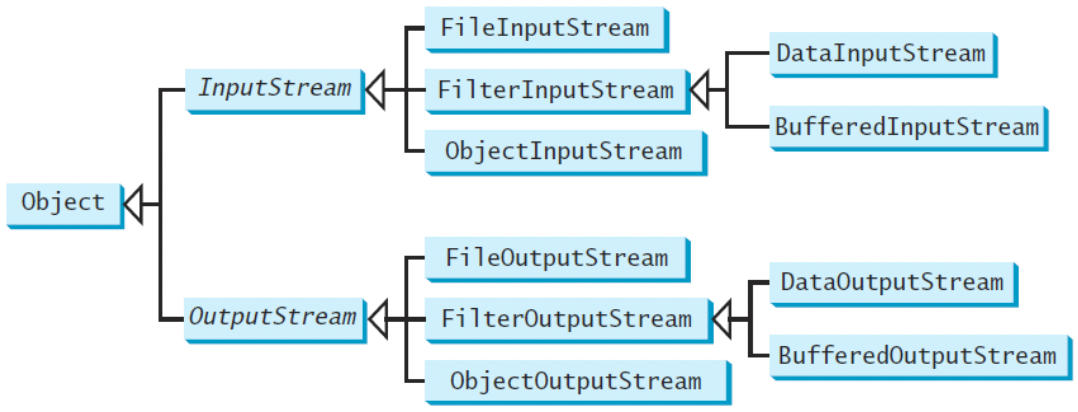
\includegraphics[scale=0.6]{IOChart}
	\end{itemize}

	\item Standard I/O
	\begin{itemize}
		\item \textbf{System.in}
		\begin{itemize}
			\item Object of type \textbf{InputStream}
			\item Typically refers to the keyboard
			\item Reading data could be done using the \textbf{Scanner} class. Its methods include:
			\begin{itemize}
				\begin{minipage}{\widthof{String nextLine()} + 1cm}
					\item \textbf{String next()}
					\item \textbf{String nextLine()}
				\end{minipage}
				\begin{minipage}{\widthof{double nextDouble()} + 1cm}
					\item \textbf{int nextInt()}
					\item \textbf{double nextDouble()}
				\end{minipage}
			\end{itemize}
		\end{itemize}

		\item \textbf{System.out}
		\begin{itemize}
			\item Object of type \textbf{PrintStream}
			\item Typically refers to the console
		\end{itemize}
	\end{itemize}

	\item The \textbf{File} class
	\begin{itemize}
		\item Contains methods for obtaining the properties of a file/directory and
		for renaming and deleting a file/directory
		\item Files could be specified using absolute or relative names
		\item Constructing a \textbf{File} instance does not create a file on the machine
		\item Methods include:
		\begin{itemize}
			\begin{minipage}[t]{\widthof{\textbf{boolean createNewFile()}} + 1cm}
				\item \textbf{boolean createNewFile()}
				\item \textbf{boolean delete()}
				\item \textbf{boolean exists()}
			\end{minipage}
			\begin{minipage}[t]{\widthof{\textbf{boolean isDirectory()}} + 1cm}
				\item \textbf{boolean isDirectory()}
				\item \textbf{File [] listFiles()}
			\end{minipage}
		\end{itemize}
	\end{itemize}

	\item File I/O
	\begin{itemize}
		\item Reading could be done using the \textbf{Scanner} class
		\begin{itemize}
			\item e.g. \textbf{Scanner input = new Scanner(new File(filename));}
		\end{itemize}
		\item Writing could be done using the \textbf{FileWrite} class
		\begin{itemize}
			\item e.g. \textbf{FileWriter output = new FileWriter(filename, append);}
		\end{itemize}
	\end{itemize}

	\newpage

	\item Regular Expressions
	\begin{itemize}
		\item A regular expression (abbreviated regex) is a string that describes a pattern for matching a set of strings.
		\item Regular expressions provide a simple and effective way to validate user input
		\begin{itemize}
			\item e.g. phone numbers
		\end{itemize}
		\item Java supports regular expressions using the \textbf{java.util.regex} package
		\item The \textbf{Pattern} class can be used to define the pattern
		\begin{itemize}
			\item The \textbf{compile} method takes a string representing the regular expression as an argument and compiles it into a pattern
		\end{itemize}
		\item The \textbf{Matcher} class can be used to search for the pattern. Its methods include:
		\begin{itemize}
			\item \textbf{boolean find()}
			\item \textbf{boolean matches()}
		\end{itemize}
		\item Example
		\begin{Verbatim}
	Pattern pattern = Pattern.compile("H.*d");
	Matcher matcher = pattern.matcher("Hello World");
	System.out.println(matcher.matches());
		\end{Verbatim}
	\end{itemize}

	\item Commonly Used Regular Expressions\\
	\begin{tabular}{l l l}
		\hline
		\textit{Regular Expression} & \textit{Matches} & \textit{Example}\\
		\hline
		\hline
		\texttt{.} & any single character & \texttt{Java} matches \texttt{J..a}\\
		\texttt{(ab|cd)} & \texttt{ab} or \texttt{cd} & \texttt{ten} matches \texttt{t(en|im)}\\
		\texttt{[abc]} & \texttt{a}, \texttt{b}, or \texttt{c} & \texttt{Java} matches \texttt{Ja[uvwx]a}\\
		\texttt{[\string^abc]} & any character except \texttt{a}, \texttt{b}, or \texttt{c} & \texttt{Java} matched \texttt{Ja[\string^ars]a}\\
		\texttt{[a-z]} & \texttt{a} through \texttt{z} & \texttt{Java} matches \texttt{[A-M]av[a-d]}\\
		\texttt{[\string^a-z]} & any character except \texttt{a} through \texttt{z} & \texttt{Java} matches \texttt{J]av[\string^b-d]}\\
		\texttt{[a-e[m-p]]} & \texttt{a} through \texttt{e} or \texttt{m} through \texttt{p} & \texttt{Java} matches \texttt{[A-G[I-M]]av[a-d]}\\
		\texttt{[a-e\&\&[c-p]] }& intersection of \texttt{a-e} with \texttt{c-p} & \texttt{Java} matches \texttt{[A-P\&\&[I-M]]av[a-d]}\\
		\texttt{\textbackslash d} & a digit, same as \texttt{[0-9]} & \texttt{Java2} matches ``\texttt{Java[\textbackslash\textbackslash d]}'' \\
		\texttt{\textbackslash D} & a non-digit & \texttt{\$Java} matches ``\texttt{[\textbackslash\textbackslash D][\textbackslash\textbackslash D]ava}"\\
		\texttt{\textbackslash w} & a word character & \texttt{Java1} matches ``\texttt{[\textbackslash\textbackslash w]ava[\textbackslash\textbackslash w]}"\\
		\texttt{\textbackslash W} & a non-word character & \texttt{\$Java } matches ``\texttt{[\textbackslash\textbackslash W][\textbackslash\textbackslash w]ava}"\\
		\texttt{\textbackslash s} & a whitespace character & ``\texttt{Java 2}'' matches ``\texttt{Java\textbackslash\textbackslash s2}"\\
		\texttt{\textbackslash S} & a non-whitespace character & \texttt{Java} matches ``\texttt{[\textbackslash\textbackslash S]ava}"\\
		\hline
		\texttt{\emph{p*}} & zero or more occurrences of pattern \texttt{\emph{p}} & \makecell[cc]{\texttt{aaaabb} matches ``\texttt{a*bb}" \\ \texttt{ababab} matches ``\texttt{(ab)*}"}\\
		\hline
		\texttt{\emph{p+}} & one or more occurrences of pattern \texttt{\emph{p}} & \makecell[cc]{\texttt{a} matches ``\texttt{a+b*}" \\ \texttt{able} matches ``\texttt{(ab)+.*}"}\\
		\hline
		\texttt{\emph{p?}} & zero or one occurrence of pattern \texttt{\emph{p}} & \makecell[cc]{\texttt{Java} matches ``\texttt{J?Java}" \\ \texttt{Java} matches ``\texttt{J?ava}"}\\
		\hline
		\texttt{\emph{p\{n\}}} & exactly \texttt{n} occurrences of pattern \texttt{\emph{p}} & \makecell[cc]{\texttt{Java} matches ``\texttt{J\{1\}.*}" \\ \texttt{Java} does not match ``\texttt{.\{2\}}"}\\
		\hline
		\texttt{\emph{p\{n,\}}} & at least \texttt{n} occurrences of pattern \texttt{\emph{p}} & \makecell[cc]{\texttt{aaaa} matches ``\texttt{a\{1,\}}" \\ \texttt{a} does not match ``\texttt{a\{2,\}}"}\\
		\hline
		\texttt{\emph{p\{n, m\}}} & between \texttt{n} and \texttt{m} occurrences (inclusive) & \makecell[cc]{\texttt{aaaa} matches ``\texttt{a\{1,9\}}" \\ \texttt{abb} does not match ``\texttt{a\{2,9\}bb}"}\\
	\end{tabular}

\end{itemize}


%\end{document}
\newpage
%\input{preamble.txt}
%
%\begin{document}
\section{Introduction to Android}
\begin{itemize}
	\item Android
	\begin{itemize}
		\item Android is a platform comprising of three components
		\begin{itemize}
			\item An operating system
			\item A framework for developing applications
			\item Devices that run the Android operating system and the applications created
			for it
		\end{itemize}
		\item Android SDK
		\begin{itemize}
			\item A collection of libraries and tools that are needed for developing Android applications
		\end{itemize}
		\item Android Studio
		\begin{itemize}
			\item IDE for Android application development
		\end{itemize}
	\end{itemize}

	\item Android App Basics
	\begin{itemize}
		\item An Android app is a collection of screens, and each screen is comprised of a layout and an activity
		\begin{itemize}
			\item Layout: describes the appearance of a screen (written in XML)
			\item Activity: responsible for managing user interaction with the screen (written in java)
		\end{itemize}
		\item Folder structure:
		\begin{itemize}
			\begin{minipage}[t]{0.15\textwidth}
				\item Manifest file
				\item Java file
			\end{minipage}
			\begin{minipage}[t]{0.3\textwidth}
				\item Resource files
				\item Gradle scripts
			\end{minipage}
		\end{itemize}
	\end{itemize}
	\item The Manifest file
	\begin{itemize}
		\item It defines the structure and metadata of an application, its components, and its requirements
		\item Stored in the root of its project hierarchy as an XML file
	\end{itemize}

	\item Resources and resource IDs
	\begin{itemize}
		\item Resources are maintained in sub-directories of the \Verb|app/res| directory
		\begin{itemize}
			\item \Verb|res/layout|
			\item \Verb|res/values|
			\item Etc.
		\end{itemize}
		\item A resource can be accessed in the code using its resource ID (e.g. \Verb|R.layout.activity_main|)
		\begin{itemize}
			\item Android uses \Verb|R.java| to keep track of the resources used within the app
		\end{itemize}
	\end{itemize}

	\item View
	\begin{itemize}
		\item Most GUI components are instances of the \textbf{View} class or one of its subclasses
		\begin{itemize}
			\item e.g. Button, EditText, ImageView, etc.
		\end{itemize}
		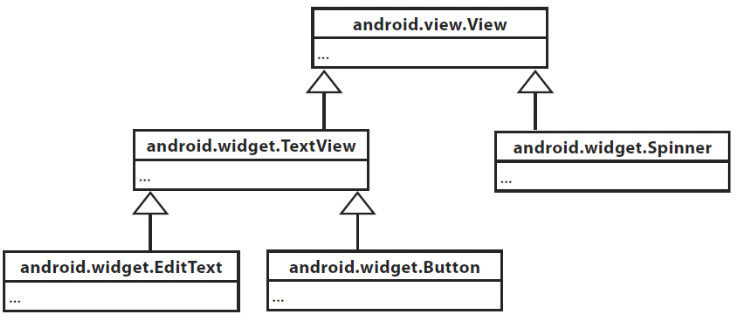
\includegraphics[scale=0.7]{View.png}
	\end{itemize}

	\newpage
	\item View Group
	\begin{itemize}
		\item A special type of view that can contain other views
		\item A layout is a type of view group\\
		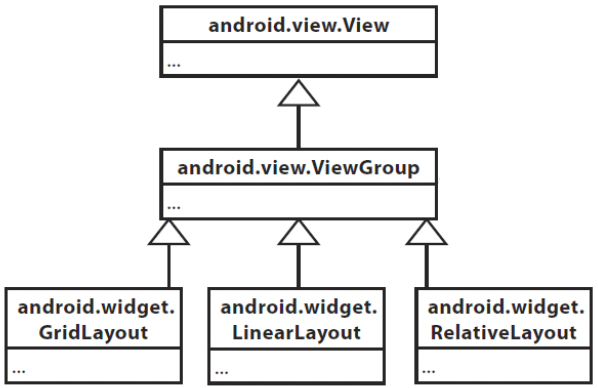
\includegraphics[scale=0.7]{ViewGroup.png}
	\end{itemize}

	\item Common GUI compnents
	\begin{itemize}
		\begin{minipage}[t]{0.15\textwidth}
			\item TextView
			\item EditText
			\item Button
		\end{minipage}
		\begin{minipage}[t]{0.15\textwidth}
			\item Switch
			\item Spinner
			\item Toast
		\end{minipage}
	\end{itemize}

	\item Intents
	\begin{itemize}
		\item An intent is an object that can be used to bind activities together at runtime
		\begin{itemize}
			\item If one activity wants to start a second activity, it does it by sending an intent to Android. Android will start the second activity and pass it the intent
		\end{itemize}
		\item Data can be passed between activities using intent extras
		\begin{itemize}
			\item e.g. \Verb|intent.putExtra("message", value);|
		\end{itemize}
	\end{itemize}
\end{itemize}

%\end{document}
\newpage
%\input{preamble.txt}

%\begin{document}
\section{Android -- Storing Data}
\begin{itemize}
	\item Data storage options
	\begin{itemize}
		\item File system
		\item Shared preferences
		\item Databases
		\begin{itemize}
			\item e.g. SQLite, Firebase Realtime Database
		\end{itemize}
	\end{itemize}

	\item File system
	\begin{itemize}
		\item Android’s file system consists of six main partitions
		\begin{itemize}
			\begin{minipage}[t]{0.15\textwidth}
				\item \Verb|/boot|
				\item \Verb|/system|
			\end{minipage}
			\begin{minipage}[t]{0.15\textwidth}
				\item \Verb|/recovery|
				\item \Verb|/data|
			\end{minipage}
			\begin{minipage}[t]{0.15\textwidth}
				\item \Verb|/cache|
				\item \Verb|/misc|
			\end{minipage}
		\end{itemize}
		\item Reading/writing data to a file on internal storage can be done using
		\begin{itemize}
			\begin{minipage}[t]{0.23\textwidth}
				\item \Verb|openFileInput()|
			\end{minipage}
			\begin{minipage}[t]{0.2\textwidth}
				\item \Verb|openFileOutput()|
			\end{minipage}
		\end{itemize}
	\end{itemize}

	\item Shared preferences
	\begin{itemize}
		\item Suitable for simple data that could be stored as key/value pairs
		\item A \textbf{SharedPreferences} object refers to a file containing key/value pairs and provides methods to read and write them
		\item Creating/accessing shared preference files can be done using:
		\begin{itemize}
			\begin{minipage}[t]{0.23\textwidth}
				\item \Verb|getPreferences()|
			\end{minipage}
			\begin{minipage}[t]{0.3\textwidth}
				\item \Verb|getSharedPreferences()|
			\end{minipage}
		\end{itemize}
	\end{itemize}

	\item SQLite
	\begin{itemize}
		\begin{minipage}[t]{0.22\textwidth}
			\item Relational database
			\item Serverless
		\end{minipage}
		\begin{minipage}[t]{0.22\textwidth}
			\item Zero-configuration
			\item File-based
		\end{minipage}
		\begin{minipage}[t]{0.15\textwidth}
			\item Widely used
		\end{minipage}
	\end{itemize}

	\item Firebase Realtime Database
	\begin{itemize}
		\item Cloud-hosted
		\item Employs data synchronization
		\begin{itemize}
			\item Every time data changes, all connected clients automatically receive updates
		\end{itemize}
		\item NoSQL
		\begin{itemize}
			\item Data is stored as JSON
		\end{itemize}
		\item The Firebase SDK provides many classes and methods to store and sync data. E.g.
		\begin{itemize}
			\begin{minipage}[t]{0.24\textwidth}
				\item \Verb|DatabaseReference|
				\item \Verb|DataSnapshot|
			\end{minipage}
			\begin{minipage}[t]{0.22\textwidth}
				\item \Verb|ValueEventListener|
			\end{minipage}
		\end{itemize}
	\end{itemize}

	\item JSON
	\begin{itemize}
		\item \textbf{J}ava\textbf{S}cript \textbf{O}bject \textbf{N}otation
		\item Language-independent
		\item Supported by many programming languages
		\item Uses readable text to represent data in the form of key/value pairs
		\item Example \begin{Verbatim}
			{
				"name": "Alex”,
				"age”: 25,
				"address”: {
					"country”: "Canada”,
					"city”: "Toronto”
				}
			}
		\end{Verbatim}

	\end{itemize}
\end{itemize}

%\end{document}

\newpage
%\input{preamble.txt}

%\begin{document}
	\section{Android  -- Testing}
	\begin{itemize}
		\item Model-View-Presenter
		\begin{itemize}
			\vspace{0.2cm}
			\begin{minipage}[b]{0.65\textwidth}
				\item An architectural design pattern that results in code that is easier to test
				\item It consists of three components:
				\begin{enumerate}
					\item Model (Data)
					\item View (UI)
					\item Presenter (Business logic)
				\end{enumerate}
			\end{minipage}
			\begin{minipage}[t]{0.2\textwidth}
				\vspace{-3.5cm}
				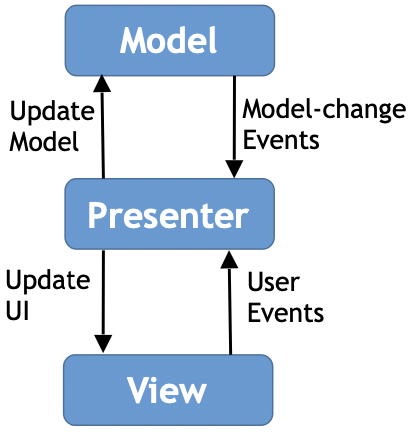
\includegraphics[scale=0.6]{MVP.png}
			\end{minipage}
		\end{itemize}

		\item Local and Instrumented Tests
		\begin{itemize}
			\vspace{0.2cm}
			\begin{minipage}[b]{0.5\textwidth}
				\item Local unit tests
				\begin{itemize}
					\item Run on the machine’s local JVM
					\item Do not depend on the Android framework
				\end{itemize}
				\item Instrumented tests
				\begin{itemize}
					\item Run on an actual device or an emulator
					\item Usually used for integration and UI tests
				\end{itemize}
			\end{minipage}
			\begin{minipage}[t]{0.4\textwidth}
				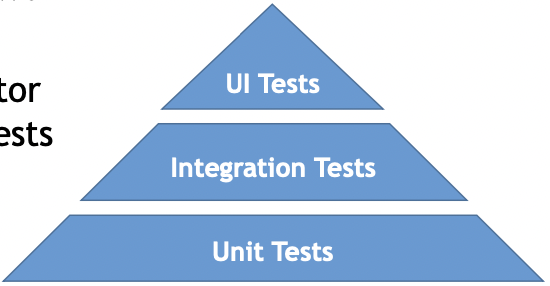
\includegraphics[scale=0.7]{LITests.png}
			\end{minipage}
		\end{itemize}

		\item Commonly used tools
		\begin{itemize}
			\item JUnit
			\begin{itemize}
				\item Writing unit tests
			\end{itemize}
			\item Mockito
			\begin{itemize}
				\item Creating dummy (mock) objects to facilitate testing a component in
				isolation
			\end{itemize}
			\item Roboelectric
			\begin{itemize}
				\item Running tests that involve the Android framework without an emulator or a device
			\end{itemize}
			\item Espresso
			\begin{itemize}
				\item Writing UI tests
			\end{itemize}
		\end{itemize}

		\item Mock Objects
		\begin{itemize}
			\item A mock is software component that is used to replace the “real” component during testing
			\item Mock objects could be used to:
			\begin{itemize}
				\item Represent components that have not yet been implemented
				\item Speed up testing
				\item Reduce the cost
				\item Avoid unrecoverable actions
				\item Etc.
			\end{itemize}
		\end{itemize}

		\item Mockito
		\begin{itemize}
			\item A mocking framework for Java
			\item Features include:
			\begin{itemize}
				\item Creating mocks
				\item Stubbing
				\item Verifying behavior
			\end{itemize}
		\end{itemize}
	\end{itemize}

%\end{document}

\end{document}

